% \section{Análisis y discusión de los resultados}
% En esta sección se presentan los resultados obtenidos durante la investigación para el desarrollo del
% presente proyecto. Aquí se describen los procesos realizados para el envío de alertas de emergencia con
% ubicación en tiempo real (datos georreferenciados), basados en las respuestas obtenidas de las entrevistas
% realizadas en el capítulo anterior, así como la medición de la precisión de dichos datos georreferenciados.


\section{Análisis del proceso actual}
A continuación se describe el proceso para reportar incidentes por parte de los ciudadanos a través del servicio
de emergencia Ecu 911. Este proceso se basa en la información obtenida de la entrevista realizada al teniente
coronel de estado mayor Christian Iván Quintana Guerra, En la Figura 1 se detalla el siguiente proceso, donde:

\begin{enumerate}
    \item El usuario llama al número de emergencia del ECU 911.
    \item El operador recibe la llamada y solicita la información necesaria al usuario.
    \item En base al tipo de incidente, el operador asigna la emergencia a la entidad correspondiente.
    \item La entidad correspondiente recibe la emergencia y envía una unidad al lugar del incidente.
    \item La unidad llega al lugar del incidente, donde:
          \begin{enumerate}
              \item La unidad verifica la información con la que cuenta:
                    \begin{enumerate}
                        \item Si cuenta con la información necesaria, la emergencia es atendida.
                        \item Si no cuenta con la información necesaria, se solicita a la víctima o testigo la información faltante.
                    \end{enumerate}
          \end{enumerate}
    \item Se reporta el incidente la atención de la emergencia y la información es almacenada en una matriz de excel.
\end{enumerate}

\begin{figure}[H]
    \centering
    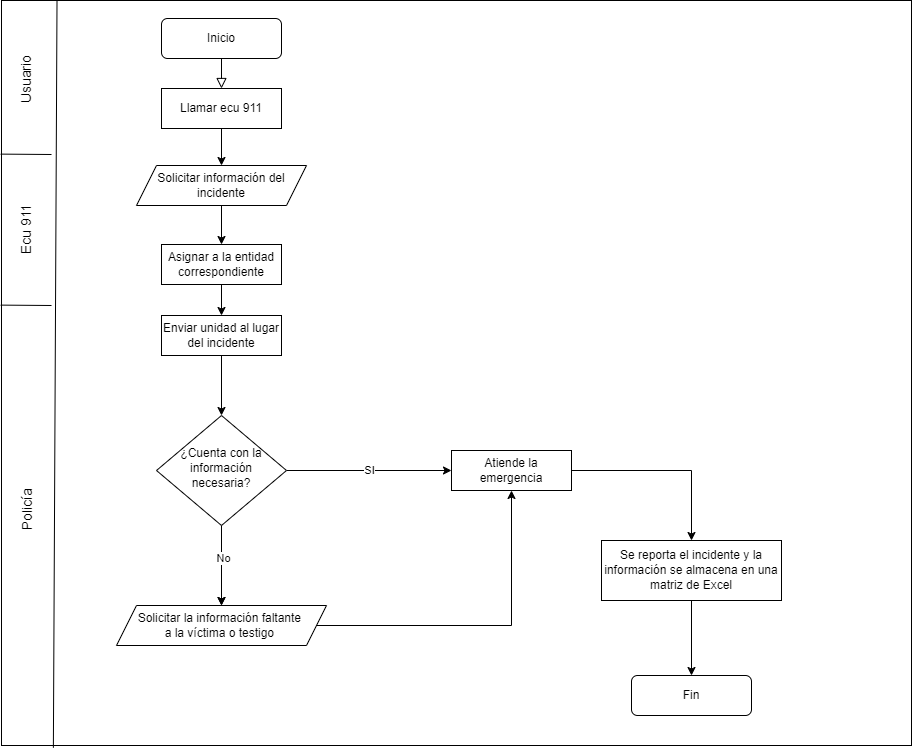
\includegraphics[width=0.8\textwidth]{chapters/III-resultados-y-discusion/resources/images/proceso-actual.png}
    \caption{Proceso actual de reporte de incidentes al ECU 911.}
    \label{fig:proceso-actual}
\end{figure}


\subsection{Análisis de herramientas de desarrollo}
En este apartado se presenta el análisis y selección de las herramientas de desarrollo que se utilizarán para la
implementación del proyecto.

\section{Análisis y selección de la metodología de desarrollo}

En la Tabla \ref{tab:metodologias} se presenta una comparación entre las metodologías de desarrollo de software ágil
y tradicional. Se evalúan aspectos como el estilo de gestión, la gestión del conocimiento, el modelo de desarrollo,
la estructura organizativa y el control de calidad, entre otros. En este análisis, se destaca que la metodología ágil
es la más adecuada para el desarrollo del proyecto actual. Esta metodología permite realizar cambios en el desarrollo
del software de manera rápida y eficiente, además de adaptarse fácilmente a equipos de desarrollo pequeños y medianos,
manteniendo una planificación y control de calidad permanente en iteraciones a corto plazo. En contraposición, la
metodología tradicional requiere una planificación exhaustiva y detallada, lo cual no es apropiado para el desarrollo
de software adaptativo de alta calidad en equipos pequeños. Esto se debe a que la metodología tradicional presupone
que los sistemas sean completamente definidos y predecibles, y cualquier cambio en el desarrollo puede resultar en
un alto costo de reinicio.

\bigbreak
Por consiguiente, se optó por la metodología ágil para el desarrollo del presente proyecto.

\begin{longtable}{|p{5cm}|p{5cm}|p{5cm}|}
    \caption[Análisis y comparación entre metodologías de desarrollo de software ágil y tradicional]{Análisis y comparación entre metodologías de desarrollo de software ágil y tradicional \cite{stoicaSoftwareDevelopmentAgile2013}.} \label{tab:metodologias}                                                                                                                              \\

    \hline \multicolumn{1}{|c|}{\textbf{Criterio}} & \multicolumn{1}{|c|}{\textbf{Metodología tradicional}}                                                                             & \multicolumn{1}{|c|}{\textbf{Metodología ágil}}                                                                                                                                                     \\ \hline
    \endfirsthead

    \multicolumn{3}{c}%
    {{\normalfont \tablename\ \thetable{} -- continuación de la página anterior}}                                                                                                                                                                                                                                                                                                             \\
    \hline \multicolumn{1}{|c|}{\textbf{Criterio}} & \multicolumn{1}{|c|}{\textbf{Metodología tradicional}}                                                                             & \multicolumn{1}{|c|}{\textbf{Metodología ágil}}                                                                                                                                                     \\ \hline
    \endhead

    \hline \multicolumn{3}{|r|}{{Continua en la siguiente página}}                                                                                                                                                                                                                                                                                                                            \\ \hline
    \endfoot

    \hline \hline
    \endlastfoot
    Hipótesis fundamental                          & Los sistemas pueden ser completamente definidos, predecibles y se construyen a través de una planificación exhaustiva y detallada. & Pequeños equipos emplean el principio de mejorar constantemente el diseño y realizar pruebas basadas en una retroalimentación rápida y cambios para desarrollar software adaptativo de alta calidad \\\hline
    Estilo de gestión                              & Mando y control                                                                                                                    & Liderazgo y colaboración                                                                                                                                                                            \\\hline
    Gestión del conocimiento                       & Explicito                                                                                                                          & Tácito                                                                                                                                                                                              \\\hline
    Comunicación                                   & Formal                                                                                                                             & Informal                                                                                                                                                                                            \\\hline
    Modelo de desarrollo                           & Modelo de ciclo de vida (cascada, espiral o modelos modificados)                                                                   & Modelo de entrega evolutivo                                                                                                                                                                         \\\hline
    Estructura organizativa                        & Mecánica (burocrática, alta formalización), dirigida a grandes organizaciones                                                      & Orgánica (flexible y participativa, fomenta la cooperación social), dirigida a pequeñas y medianas organizaciones                                                                                   \\\hline
    Control de calidad                             & Planificación difícil y control estricto. Pruebas difíciles y tardías                                                              & Control permanente o requisitos, diseño y soluciones. Pruebas permanentes                                                                                                                           \\\hline
    Requisitos de los usuarios                     & Detallado y definido antes de la codificación/implantación                                                                         & Entrada interactiva                                                                                                                                                                                 \\\hline
    Coste del reinicio                             & Alto                                                                                                                               & Bajo                                                                                                                                                                                                \\\hline
    Dirección del desarrollo                       & Fijo                                                                                                                               & Fácil de cambiar                                                                                                                                                                                    \\\hline
    Pruebas                                        & Una vez finalizada la codificación                                                                                                 & Cada iteración                                                                                                                                                                                      \\\hline
    Participación del cliente                      & Baja                                                                                                                               & Alta                                                                                                                                                                                                \\\hline
    Requisitos                                     & Muy estable, conocido de antemano                                                                                                  & Emergente, con cambios rápidos                                                                                                                                                                      \\\hline
    Arquitectura                                   & Diseño para necesidades actuales y previsibles                                                                                     & Diseño para las necesidades actuales                                                                                                                                                                \\\hline
    Remodelación                                   & Caro                                                                                                                               & No es caro                                                                                                                                                                                          \\\hline
    Tamaño                                         & Grandes equipos y proyectos                                                                                                        & Pequeños equipos y proyectos                                                                                                                                                                        \\
    Objetivos principales                          & Alta seguridad                                                                                                                     & Valor rápido                                                                                                                                                                                        \\
\end{longtable}

Con el objetivo de seleccionar la metodología ágil más adecuada para el desarrollo del proyecto, se realizó un
análisis comparativo entre las metodologías ágiles tomando en cuenta criterios tales como, los cuales se detallan en
la Tabla \ref{tab:metodologias-agiles}.

\begin{longtable}{|p{2.5cm}|p{3cm}|p{3cm}|p{3cm}|}
    \caption{Análisis y comparación entre metodologías de desarrollo ágil} \label{tab:metodologias-agiles}                                                                                                                                                                                                                                                                                                                                                                                                                                                                                                \\

    \hline \multicolumn{1}{|c|}{\textbf{Criterio}} & \multicolumn{1}{|c|}{\textbf{XP}}                                                                                                                                   & \multicolumn{1}{|c|}{\textbf{Kanban}}                                                                                                                                                   & \multicolumn{1}{|c|}{\textbf{Scrum}}                                                                                                                                                 \\ \hline
    \endfirsthead

    \multicolumn{4}{c}%
    {{\normalfont \tablename\ \thetable{} -- continuación de la página anterior}}                                                                                                                                                                                                                                                                                                                                                                                                                                                                                                                         \\
    \hline \multicolumn{1}{|c|}{\textbf{Criterio}} & \multicolumn{1}{|c|}{\textbf{XP}}                                                                                                                                   & \multicolumn{1}{|c|}{\textbf{Kanban}}                                                                                                                                                   & \multicolumn{1}{|c|}{\textbf{Scrum}}                                                                                                                                                 \\ \hline
    \endhead

    \hline \multicolumn{4}{|r|}{{Continua en la siguiente página}}                                                                                                                                                                                                                                                                                                                                                                                                                                                                                                                                        \\ \hline
    \endfoot

    \hline \hline
    \endlastfoot
    Tamaño del proyecto                            & Pequeños y medianos.                                                                                                                                                & Pequeños, medianos y grandes.                                                                                                                                                           & Proyectos de toda magnitud y dificultad.                                                                                                                                             \\ \hline
    Tamaño del equipo                              & 5 o menos integrantes.                                                                                                                                              & De 5 a 14 integrantes.                                                                                                                                                                  & De 5 a 9 integrantes.                                                                                                                                                                \\ \hline
    Enfoque                                        & Se centra en ofrecer un producto de alta calidad y en garantizar la satisfacción del cliente.                                                                       & Se centra en la mejora continua del proyecto.                                                                                                                                           & Se centra en la colaboración en equipo.                                                                                                                                              \\ \hline
    Roles                                          & Programador, cliente, tester, coach, encargado del seguimiento.                                                                                                     & No existen roles específicos, aunque algunos equipos pueden recibir apoyo de un coach.                                                                                                  & Product owner, scrum master, equipo de desarrollo.                                                                                                                                   \\ \hline
    Ciclo de vida                                  & Exploración, planificación, iteraciones, producción, monitoreo.                                                                                                     & Inicio, del inglés To-Do, Trabajo en progreso, del inglés Doing, Listo para revisión, del inglés Done.                                                                                  & Sprint, sprint panning, daily scrum, sprint review, sprint retrospective.                                                                                                            \\ \hline
    Ciclo de entrega                               & Se centra en hacer entregas regulares y de menor escala conforme se desarrollan nuevas funcionalidades.                                                             & Las tareas progresan a lo largo del tablero Kanban a medida que avanzan en el proceso de desarrollo, y una vez terminadas, se entregan directamente al cliente.                         & Al final de cada iteración o sprint, se realiza una revisión del trabajo y se entrega el avance del producto al cliente o usuario.                                                   \\ \hline
    Gestión de cambios                             & Se caracteriza por su capacidad de adaptarse a los cambios. En XP, los cambios son recibidos en todo momento debido a su enfoque en la retroalimentación constante. & Los cambios pueden ser gestionados a medida que son detectados y priorizados.                                                                                                           & Si se detecta un cambio que requiere atención, se cancela el Sprint en curso y se inicia uno nuevo con las adaptaciones necesarias.                                                  \\ \hline
    Enfoque en la calidad                          & Las pruebas unitarias, la integración continua y la refactorización son pilares esenciales en XP que contribuyen a mantener la calidad del software.                & La identificación temprana de problemas y su resolución inmediata son fundamentales para mantener la calidad. Cualquier defecto identificado es priorizado y se corregido de inmediato. & Durante un Sprint, el equipo se dedica a implementar y probar las funcionalidades según lo planificado. Cada funcionalidad debe satisfacer los criterios de aceptación establecidos. \\                                                                                                                                           & Planificación y modelado                                                                                                                                        & Rápida y flexible                                                                                                                  \\
\end{longtable}


\section{Análisis y selección de herramientas de desarrollo}

Mediante el análisis realizo en la Tabla \ref{tab:metodologias-agiles}, se optó por emplear la metodología de
Desarrollo Rápido de Aplicaciones (RAD) debido a su enfoque centrado en la rápida entrega de soluciones y
prototipos funcionales a los clientes. La selección de RAD se basa en su capacidad para proporcionar resultados
en plazos cortos gracias a su naturaleza iterativa e incremental.

\section{Análisis y selección del framework de desarrollo para el servidor web (Backend)}

Como lenguaje de desarrollo para el servidor web (Backend) se optó por utilizar Typescript junto al entorno de
ejecución de Node.js, debido que este permite el desarrollo de aplicaciones escalables y de alto rendimiento,
impulsado por eventos asíncronos, ademas del amplio soporte por parte de la comunidad y documentación disponible,
así como a la facilidad de uso y la gran cantidad de librerías y frameworks disponibles para el desarrollo de aplicaciones
web \cite{haroDesarrolloBackendPara}.
\bigbreak
Como framework de desarrollo para el servidor web (backend), se optó por el uso de NestJS debido a que proporciona
una arquitectura modular y escalable basada en el patrón de diseño de inyección de dependencias. Además, combina
elementos de la programación orientada a objetos (POO), programación funcional (PF) y programación funcional
reactiva (PFR). NestJS permite utilizar como base dos de los frameworks más populares en el desarrollo web, Express y
Fastify, mediante un nivel de abstracción superior que permite exponer las APIs de ambos frameworks de forma
directa al desarrollador, lo que proporciona una mayor flexibilidad al momento de incluir paquetes de terceros.
Además, destaca por la gran cantidad de módulos y librerías que posee \cite{phamDEVELOPINGBACKENDWEB2020}.
\bigbreak
En la tabla \ref{tab:frameworks-backend} se presenta una comparación entre Express y Fastify tomando en cuenta
criterios como el soporte para Typescript, rendimiento, velocidad, documentación, soporte por la comunidad y
paquetes/librerías.

\begin{longtable}{|p{5cm}|p{5cm}|p{5cm}|}
    \caption[]{Análisis y comparación entre los frameworks de NodeJS Express y Fastify \cite{ExpressInfraestructuraAplicaciones}\cite{FastLowOverhead}} \label{tab:frameworks-backend}                                                                                                              \\

    \hline \multicolumn{1}{|c|}{\textbf{Criterio}} & \multicolumn{1}{|c|}{\textbf{Express.js}}                                                                                      & \multicolumn{1}{|c|}{\textbf{Fastify.js}}                                                                   \\ \hline
    \endfirsthead

    \multicolumn{3}{c}%
    {{\normalfont \tablename\ \thetable{} -- continuación de la página anterior}}                                                                                                                                                                                                                 \\
    \hline \multicolumn{1}{|c|}{\textbf{Criterio}} & \multicolumn{1}{|c|}{\textbf{Express.js}}                                                                                      & \multicolumn{1}{|c|}{\textbf{Fastify.js}}                                                                   \\ \hline
    \endhead

    \hline \multicolumn{3}{|r|}{{Continua en la siguiente página}}                                                                                                                                                                                                                                \\ \hline
    \endfoot

    \hline \hline
    \endlastfoot
    Soporte para Typescript                        & Mediante un paquete externo                                                                                                    & Hecho en TypeScript con soporte directo                                                                     \\
    Rendimiento                                    & 11080 peticiones/s                                                                                                             & 45871 peticiones/s                                                                                          \\
    Velocidad                                      & Más lento debido a su mayor cantidad de middleware y flexibilidad                                                              & Significativamente más rápido debido a su enfoque en la velocidad y eficiencia                              \\
    Documentación                                  & Documentación detallada y ampliamente utilizada                                                                                & Documentación completa y fácil de entender                                                                  \\
    Soporte por la comunidad                       & Gran soporte por parte de la comunidad al ser el framework mas usado                                                           & Cuenta con un soporte amplio por parte de su comunidad en creciente aumento                                 \\
    Paquetes/librerías                             & Permite integrar fácilmente tanto librerías propias como de terceros gracias a su arquitectura flexible y su amplia comunidad. & Tine gran soporte para incorporar librerías personalizadas y de terceros gracias a su creciente popularidad \\
\end{longtable}

Considerando el análisis presentado en la Tabla \ref{tab:frameworks-backend}, se optó por utilizar Fastify como
el framework base para NestJS. Esto se debe a que Fastify es más rápido que Express, gracias a su enfoque en la
velocidad y la eficiencia. Fastify ha sido diseñado específicamente con el objetivo de ser rápido y eficiente,
lo que lo convierte en una excelente elección para aplicaciones que necesitan un alto rendimiento.

\section{Análisis y selección del framework de desarrollo para el cliente web (Frontend)}

Dado que en el lado del servidor se ha optado por utilizar TypeScript, para el cliente web (frontend) se ha optado
por emplear el mismo lenguaje de programación. Esto se debe a que permite una integración más fluida entre el
cliente y el servidor, además de facilitar la comunicación entre ambos. Para el desarrollo del cliente web
(frontend), se han considerado tres de los frameworks más populares en la actualidad: Angular, ReactJS y VueJS.
A continuación, se presenta una comparación de estos frameworks en la Tabla \ref{tab:frameworks-web}.

\begin{longtable}{|p{3cm}|p{3cm}|p{3cm}|p{3cm}|}
    \caption[Análisis y comparación entre los frameworks Angular, ReactJS, VueJS]{Análisis y comparación entre los frameworks Angular, ReactJS, VueJS  \cite{cincovicComparisonAngularVs2020}} \label{tab:frameworks-web} \\

    \hline \multicolumn{1}{|c|}{\textbf{Criterio}} & \multicolumn{1}{|c|}{\textbf{Angular}} & \multicolumn{1}{|c|}{\textbf{ReactJS}} & \multicolumn{1}{|c|}{\textbf{VueJS}}                                               \\ \hline
    \endfirsthead

    \multicolumn{4}{c}%
    {{\normalfont \tablename\ \thetable{} -- continuación de la página anterior}}                                                                                                                                         \\
    \hline \multicolumn{1}{|c|}{\textbf{Criterio}} & \multicolumn{1}{|c|}{\textbf{Angular}} & \multicolumn{1}{|c|}{\textbf{ReactJS}} & \multicolumn{1}{|c|}{\textbf{VueJS}}                                               \\ \hline
    \endhead

    \hline \multicolumn{4}{|r|}{{Continua en la siguiente página}}                                                                                                                                                        \\ \hline
    \endfoot

    \hline \hline
    \endlastfoot
    Popularidad                                    & Estancada                              & Creciente                              & Creciente                                                                          \\\hline
    Rendimiento                                    & Mayor sobrecarga                       & Ligero                                 & Ligero                                                                             \\\hline
    Soporte de la Comunidad                        & Mediano                                & Grande                                 & Grande                                                                             \\\hline
    Curva de Aprendizaje                           & Mediana                                & Mediana                                & Baja                                                                               \\\hline
    Conocimientos necesarios                       & TypeScript                             & JSX, TSX, Hooks                        & Ninguno                                                                            \\\hline
    Migraciones                                    & Frecuentes                             & Raras                                  & Fácilmente adaptable                                                               \\\hline
    Flexibilidad                                   & Limitada                               & Grande                                 & Grande                                                                             \\
\end{longtable}

\begin{longtable}{|p{0.5cm}|p{6cm}|p{6cm}|}
    \caption[Ventajas y desventajas de Angular, ReactJS y VueJS]{Ventajas y desventajas de Angular, ReactJS y VueJS \cite{xingResearchAnalysisFrontend2019a}} \label{tab:ventajas-desventajas-frameworks-web}                                                                                                                                                                                                                                                                        \\

    \hline \multicolumn{1}{|c|}{\textbf{Framework}} & \multicolumn{1}{|c|}{\textbf{Ventajas}}                                                                                                                                                                           & \multicolumn{1}{|c|}{\textbf{Desventajas}}                                                                                                                                                                 \\ \hline
    \endfirsthead

    \multicolumn{3}{c}%
    {{\normalfont \tablename\ \thetable{} -- continuación de la página anterior}}                                                                                                                                                                                                                                                                                                                                                                                                    \\
    \hline \multicolumn{1}{|c|}{\textbf{Framework}} & \multicolumn{1}{|c|}{\textbf{Ventajas}}                                                                                                                                                                           & \multicolumn{1}{|c|}{\textbf{Desventajas}}                                                                                                                                                                 \\ \hline
    \endhead

    \hline \multicolumn{3}{|r|}{{Continua en la siguiente página}}                                                                                                                                                                                                                                                                                                                                                                                                                   \\ \hline
    \endfoot

    \hline \hline
    \endlastfoot
    ReactJS                                         & \tabitem{Emplea un DOM virtual para lograr una eficiencia máxima al actualizar nodos según sea necesario.}                                                                                                        & \tabitem{Es necesario importar bibliotecas adicionales para manejar el estado y el modelo, ya que React no incluye la arquitectura MVC de forma nativa.}                                                   \\\hline
                                                    & \tabitem{La capacidad de renderizar en el servidor es otra ventaja que este framework ofrece, especialmente adecuada para ciertos tipos de implementaciones, como las aplicaciones enfocadas en el contenido.}    & \tabitem{Aunque React permite su uso, se distancia de los enfoques basados en clases y puede presentar dificultades para aquellos que prefieren la Programación Orientada a Objetos (POO).}                \\\hline
                                                    & \tabitem{Reduce la carga de recursos del usuario mediante el respaldo de bundling y tree shaking.}                                                                                                                &                                                                                                                                                                                                            \\\hline
                                                    & \tabitem{La programación funcional facilita la creación de código que puede ser reutilizado. }                                                                                                                    &                                                                                                                                                                                                            \\\hline
                                                    & \tabitem{Ofrece ventajas en términos de SEO en comparación con Angular y Vue.js. }                                                                                                                                &                                                                                                                                                                                                            \\\hline
    Angular                                         & \tabitem{Utiliza el patrón MVVM (Modelo-Vista-Modelo de Vista), el cual permite manipular la misma colección de datos de forma independiente dentro de una misma aplicación.}                                     & \tabitem{Posee múltiples estructuras como Inyectables, Componentes, Tuberías, Módulos, entre otros, que suelen presentar un mayor nivel de complejidad para su comprensión.}                               \\\hline
                                                    & \tabitem{Su estructura y arquitectura están diseñadas específicamente para mejorar la escalabilidad de los proyectos.}                                                                                            & \tabitem{Experimenta actualizaciones continuas, incorporando mejoras nuevas y significativas de manera constante. Sin embargo, estas actualizaciones pueden plantear desafíos al adaptarse a los cambios.} \\\hline
                                                    & \tabitem{La inyección de dependencias en los componentes ayuda a mejorar la modularidad de la aplicación.}                                                                                                        &                                                                                                                                                                                                            \\\hline
                                                    & \tabitem{La programación funcional facilita la creación de código que puede ser reutilizado. }                                                                                                                    &                                                                                                                                                                                                            \\\hline
    VueJS                                           & \tabitem{Facilita la creación de modelos modulares de gran alcance que pueden renderizarse eficientemente gracias a su estructura fundamental, sin requerir esfuerzos adicionales.}                               & \tabitem{Su participación en el mercado es moderada, lo que indica que el intercambio de información en esta plataforma se encuentra en sus primeras fases de desarrollo.}                                 \\\hline
                                                    & \tabitem{Posee una alta capacidad de respuesta y ofrece una sencilla vinculación de datos entre el código HTML y JavaScript. }                                                                                    & \tabitem{Existe el riesgo de que su flexibilidad pueda ser un problema al integrarse en proyectos extensos debido a la carencia de recursos disponibles.}                                                  \\\hline
                                                    & \tabitem{Vue gestiona de forma sobresaliente la vinculación de datos bidireccional dinámica. Además, lleva a cabo la manipulación del DOM de manera coherente, lo que lo hace ideal para diversas aplicaciones. } &                                                                                                                                                                                                            \\
\end{longtable}


Tomando en cuenta el análisis de las características de cada framework, así como sus ventajas y desventajas, se
optó por el uso de ReactJS para el desarrollo del cliente web (frontend). Esto se debe a que ReactJS es una de
las librerías más populares y ampliamente utilizadas en la actualidad, lo que significa que cuenta con una gran
comunidad de desarrolladores y una amplia variedad de recursos disponibles. Además, ReactJS posee un gran
rendimiento y eficiencia gracias a su manejo eficiente del DOM virtual, lo que lo convierte en una excelente
elección para aplicaciones web que requieren una interfaz de usuario rápida y receptiva, as���� como su capacidad
de crear componentes reutilizables, lo que facilita el desarrollo de aplicaciones web complejas y escalables.

\section{Análisis y selección del framework de desarrollo para el cliente móvil (Frontend)}

Para el desarrollo del cliente móvil (frontend), se han considerado tres de los frameworks más populares en la
actualidad: React Native, Flutter y Ionic. A continuación, se presenta una comparación de estos frameworks en la
Tabla \ref{tab:frameworks-movil}.

\begin{longtable}{|p{5cm}|p{3cm}|p{3cm}|p{3cm}|}
    \caption[Análisis y comparación entre los frameworks React Native, Flutter y Xamarin]{Análisis y comparación entre los frameworks React Native, Flutter y Xamarin \cite{alferezzamoraEstudioComparativoFrameworks2018}\cite{lazoANALISISDISENOAPLICATIVO}} \label{tab:frameworks-movil}                                                                    \\

    \hline \multicolumn{1}{|c|}{\textbf{Criterio}} & \multicolumn{1}{|c|}{\textbf{React Native}}               & \multicolumn{1}{|c|}{\textbf{Flutter}}                                                                         & \multicolumn{1}{|c|}{\textbf{Xamarin}}                                                                                       \\ \hline
    \endfirsthead

    \multicolumn{4}{c}%
    {{\normalfont \tablename\ \thetable{} -- continuación de la página anterior}}                                                                                                                                                                                                                                                                              \\
    \hline \multicolumn{1}{|c|}{\textbf{Criterio}} & \multicolumn{1}{|c|}{\textbf{React Native}}               & \multicolumn{1}{|c|}{\textbf{Flutter}}                                                                         & \multicolumn{1}{|c|}{\textbf{Xamarin}}                                                                                       \\ \hline
    \endhead

    \hline \multicolumn{4}{|r|}{{Continua en la siguiente página}}                                                                                                                                                                                                                                                                                             \\ \hline
    \endfoot

    \hline \hline
    \endlastfoot
    Lanzamiento                                    & 2015                                                      & 2017                                                                                                           & 2013                                                                                                                         \\\hline
    Licencia                                       & MIT Licensed                                              & BSD                                                                                                            & MIT Licensed                                                                                                                 \\\hline
    Lenguaje                                       & JavaScript, TypeScript                                    & Dart                                                                                                           & C\#                                                                                                                          \\\hline
    Plataformas soportadas                         & Android, IOS                                              & Android, IOS                                                                                                   & Android, IOS                                                                                                                 \\\hline
    Open source                                    & Si                                                        & Si                                                                                                             & Si                                                                                                                           \\\hline
    Paradigma                                      & Declarativo                                               & Declarativo                                                                                                    & Imperativo                                                                                                                   \\\hline
    Recarga en tiempo real                         & Si                                                        & Si                                                                                                             & No                                                                                                                           \\\hline
    Recarga en vivo                                & Si                                                        & Si                                                                                                             & No                                                                                                                           \\\hline
    Administrador de paquetes                      & NPM, Yarn                                                 & Pub                                                                                                            & NuGet                                                                                                                        \\\hline
    Enfoque multiplataforma                        & Interpretado                                              & Compilado a nativo                                                                                             & Compilado a nativo                                                                                                           \\\hline
    Compatibilidad con 64bits                      & No en android                                             & Si                                                                                                             & Si                                                                                                                           \\\hline
    Portabilidad                                   & Si                                                        & No                                                                                                             & No                                                                                                                           \\\hline
    Geolocalización                                & Incluido                                                  & Mediante paquete de la comunidad                                                                               & Incluido                                                                                                                     \\\hline
    Notificaciones                                 & Mediante paquete de la comunidad                          & Mediante paquete de la comunidad                                                                               & Mediante paquete de la comunidad                                                                                             \\\hline
    Rendimiento                                    & Alto desempeño al ser un framework ligero                 & Elevada eficiencia gracias a su propio motor de renderizado                                                    & Un desempeño sólido, aunque podría beneficiarse de una capa extra de abstracción.                                            \\\hline
    Integración con APIs y Bibliotecas             & Gran cantidad de paquetes de terceros                     & Una amplia disponibilidad de bibliotecas y paquetes de terceros gracias a su comunidad en constante desarrollo & Gran cantidad de bibliotecas y recursos disponibles, especialmente diseñados para integrarse con los servicios de Microsoft. \\\hline
    Documentación                                  & Amplia documentación                                      & Documentación amplia y detallada, además  mas de gran cantidad de recursos de terceros                         & Documentación completa y abundante                                                                                           \\\hline
    Tiempo de desarrollo                           & Rápida gracias a su hot reload con cambios en tiempo real & Rápido gracias al hot reload que permite visualizar cambios en tiempo real                                     & Tiempo de desarrollo mas lento debido a la compilación                                                                       \\
\end{longtable}

Considerando el análisis realizado en la Tabla \ref{tab:frameworks-movil}, se optó por utilizar Flutter para el
desarrollo del cliente móvil (frontend). Esto se debe a que Flutter es un framework de desarrollo de aplicaciones
móviles multiplataforma creado por Google, que permite el desarrollo de aplicaciones móviles nativas de alta
calidad para Android e iOS desde una sola base de código. Flutter destaca por su rendimiento y eficiencia, gracias
a su propio motor de renderizado, lo que lo convierte en una excelente elección para aplicaciones móviles que
requieren un alto rendimiento y una interfaz de usuario rápida y receptiva. Además, Flutter cuenta con una amplia
variedad de widgets y herramientas que facilitan el desarrollo de aplicaciones móviles complejas y escalables.

\section{Análisis y selección de la base de datos}

Pra la base de datos del proyecto se han considerado dos opciones: MySQL y PostgreSQL. A continuación, se presenta
una comparación de estas bases de datos en la Tabla \ref{tab:bases-datos}.

\label{app:analisis-bases-datos}
\begin{longtable}{|p{5cm}|p{5cm}|p{5cm}|}
    \caption[Análisis y comparación entre las bases de datos MySQL y PostgreSQL]{Análisis y comparación entre las bases de datos MySQL y PostgreSQL \cite{lazoANALISISDISENOAPLICATIVO}} \label{tab:bases-datos} \\

    \hline \multicolumn{1}{|c|}{\textbf{Criterio}} & \multicolumn{1}{|c|}{\textbf{MySQL}}                                              & \multicolumn{1}{|c|}{\textbf{PostgreSQL}}                               \\ \hline
    \endfirsthead

    \multicolumn{3}{c}%
    {{\normalfont \tablename\ \thetable{} -- continuación de la página anterior}}                                                                                                                                \\
    \hline \multicolumn{1}{|c|}{\textbf{Criterio}} & \multicolumn{1}{|c|}{\textbf{MySQL}}                                              & \multicolumn{1}{|c|}{\textbf{PostgreSQL}}                               \\ \hline
    \endhead

    \hline \multicolumn{3}{|r|}{{Continua en la siguiente página}}                                                                                                                                               \\ \hline
    \endfoot

    \hline \hline
    \endlastfoot
    GUI                                            & MySQL Workbench                                                                   & pgAdmin                                                                 \\\hline
    Consumo de recursos                            & Consumo mayor de CPU y memoria                                                    & Consumo mayor de CPU y memoria                                          \\\hline
    Tiempo de respuesta de CRUD                    & Bajo                                                                              & Alto                                                                    \\\hline
    Lenguaje de ejecución                          & C/C++                                                                             & C                                                                       \\\hline
    herencia de tablas                             & No                                                                                & Si                                                                      \\\hline
    Tipos de datos                                 & Solo tipos estándar                                                               & Estándar, store, arreglos, geográficos, definido por el usuario, etc.   \\\hline
    APIs y otros métodos de acceso                 & ADO.NET, JDBC, biblioteca C nativa, ODBC, API de transmisión para objetos grandes & ADO.NET, JDBC, ODBC, API nativa patentada                               \\\hline
    Tipos de conexión                              & Las conexiones son subprocesos del sistema operativo                              & Las conexiones son subprocesos del sistema operativo                    \\\hline
    Respaldo                                       & En MySQL, Mysqldump y XtraBackup, las herramientas proporcionan respaldo          & PostgreSQL proporciona una copia de seguridad completa en línea.        \\\hline
    Lenguajes soportados                           & C/C++, PHP, Java, Go, Delphi, Lisp, Erlang, Node.js, R, Perl, PHP                 & Go, C/C++, Java, Delphi, Javascript, Erlang, Lisp, R, .Net, Tcl, Python \\\hline
    Sistemas Operativos Soportados                 & Windows, Linux, macOS, Oracle Solaris, Fedora, FreeBSD                            & Windows, macOS, BSD, Linux, Solaris                                     \\
\end{longtable}

Tomando en cuenta el análisis presentado en la Tabla \ref{tab:bases-datos}, se optó por utilizar PostgreSQL como
la base de datos del proyecto. Esto se debe a que PostgreSQL es un sistema de gestión de bases de datos relacional
de código abierto y de alto rendimiento, que ofrece una amplia variedad de características y funcionalidades
avanzadas, como soporte para tipos de datos geoespaciales, herencia de tablas, tipos de datos definidos por el
usuario, entre otros. Además, PostgreSQL cuenta con una arquitectura robusta y escalable, que permite gestionar
grandes volúmenes de datos de forma eficiente y fiable, lo que lo convierte en una excelente elección para
aplicaciones que requieren una base de datos potente y confiable.

\section{Análisis de la precisión de los datos georreferenciados}

Con la finalidad de evaluar la precisión de los datos georreferenciados obtenidos a través de la aplicación móvil, se
desarrolló un prototipo de aplicación que permite obtener la ubicación del dispositivo móvil y compararla con un punto
de referencia conocido, el cual será seleccionado en la aplicación de prueba. Para ello, se utilizó el GPS del dispositivo
móvil para obtener la ubicación, el framework de desarrollo Flutter para la creación de la aplicación móvil y Google Maps
para la visualización de la ubicación en un mapa interactivo.
\bigbreak

En la Figura  \ref{fig:prototipo-georreferenciacion} se muestra el prototipo de la aplicación móvil desarrollada para la
evaluación de la precisión de los datos georreferenciados. Esta aplicación cuenta con un botón que permite obtener la ubicación
actual del dispositivo móvil. Con esto, el usuario puede seleccionar un punto de referencia en el mapa y guardar ambos puntos
para su posterior comparación.

\begin{figure}[H]
    \centering
    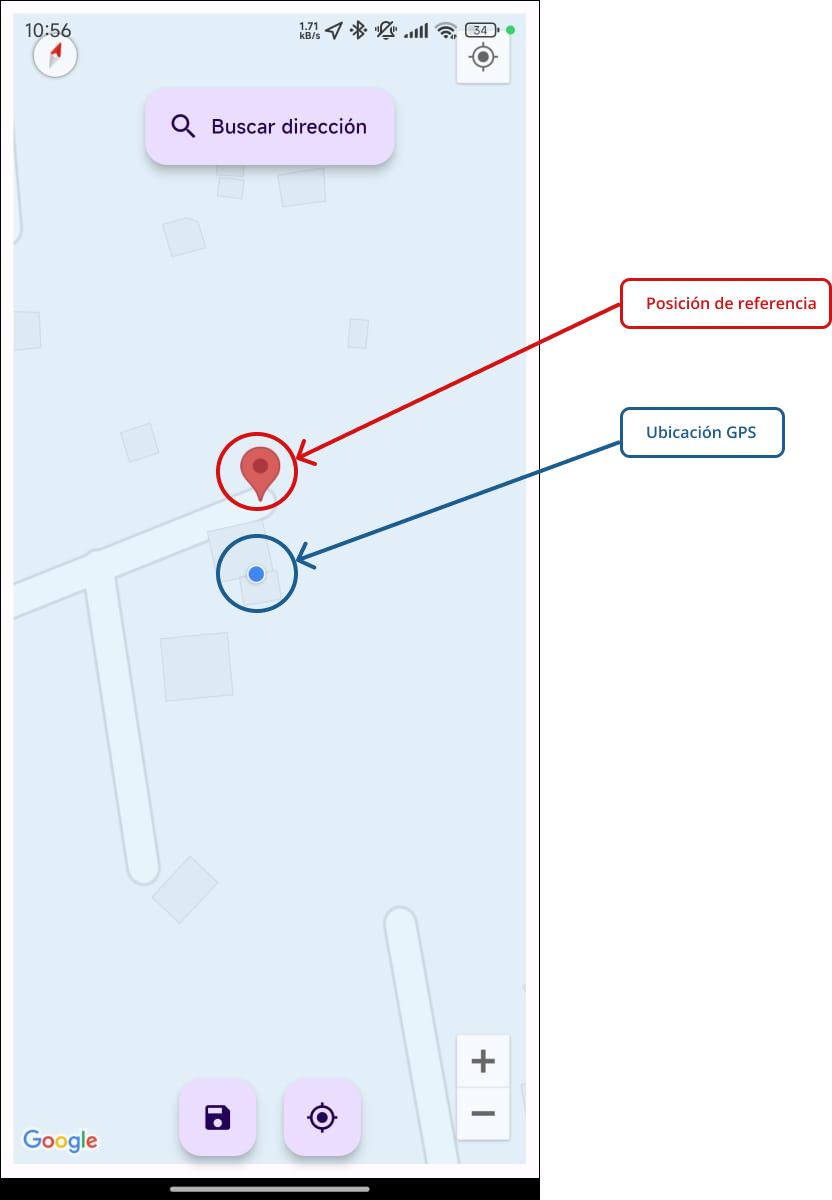
\includegraphics[width=0.3\textwidth]{chapters/III-resultados-y-discusion/resources/images/prototipo-georreferenciacion.png}
    \caption{Prototipo de la aplicación móvil para la evaluación de la precisión de los datos georreferenciados.}
    \label{fig:prototipo-georreferenciacion}
\end{figure}

Para establecer la cantidad de datos necesarios para la evaluación de la precisión de los datos georreferenciados, se optó por
utilizar una muestra infinita con población desconocida, aplicando la Ecuación \ref{eq:ecuacion-muestra-datos-georreferenciados}, donde:

\begin{itemize}
    \item n = tamaño de la muestra
    \item Z = nivel de confianza
    \item p = probabilidad de éxito o proporción esperada
    \item q = probabilidad de fracaso
    \item pq = varianza de la población
    \item e = error de estimación máximo aceptable
\end{itemize}

\begin{equation}
    n=\frac{Z^2 \cdot p \cdot q}{e^2}
    \label{eq:ecuacion-muestra-datos-georreferenciados}
\end{equation}

Sustituyendo los valores en la Ecuación \ref{eq:ecuacion-muestra-datos-georreferenciados}, se obtiene:

\begin{itemize}
    \item Z = 1.96, con un nivel de confianza del 95\% y un error de estimación máximo aceptable del 5\%
    \item p = 0.50
    \item q = 0.50
    \item e = 0.05
\end{itemize}

\begin{equation}
    n=\frac{(1.96)^2 \cdot 0.50 \cdot 0.50}{(0.05)^2}
    \label{eq:ecuacion-valores-muestra-datos-georreferenciados}
\end{equation}

\begin{equation}
    n=384.16 \approx 385
    \label{eq:ecuacion-resultado-muestra-datos-georreferenciados}
\end{equation}

Utilizando un nivel de confianza del 95\% y un error de estimación máximo aceptable del 5\%, se obtiene una muestra aproximada
de 385 puntos de referencia para la evaluación de la precisión de los datos georreferenciados.
\bigbreak

Los datos obtenidos de la aplicación móvil se almacenaron en una tabla de una base de datos PostgreSQL, la cual se muestra en
la Figura \ref{fig:tabla-georreferenciacion}. Esta tabla contiene la información de los puntos de referencia seleccionados en
la aplicación móvil, los cuales son: latitud y longitud real (Punto de referencia) y latitud y longitud obtenida mediante
GPS (Punto de ubicación).

\begin{figure}[H]
    \centering
    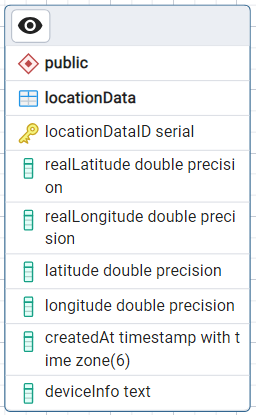
\includegraphics[width=0.3\textwidth]{chapters/III-resultados-y-discusion/resources/images/tabla-georreferenciacion.png}
    \caption{Tabla de datos georreferenciados almacenados en la base de datos PostgreSQL.}
    \label{fig:tabla-georreferenciacion}
\end{figure}

Estos datos se traspasaron a un archivo de Excel para su posterior análisis. Para ello, se utilizó un script con
Node.js y la librería de manejo de archivos ExcelJS, como se muestra en la Figura \ref{fig:script-exceljs}. La distancia entre
los puntos de referencia y los puntos de ubicación se calculó utilizando la fórmula de Haversine, dado que esta toma en cuenta
la curvatura de la Tierra y proporciona una mejor precisión \cite{basyirDeterminationNearestEmergency2017}. La función de
Haversine utilizada se muestra en la Figura \ref{fig:script-haversine}.

\begin{figure}[H]
    \begin{minted}[fontsize=\footnotesize, linenos, breaklines, frame=single]{js}
import Exceljs from "exceljs";
import distances from "./distances.json" with { type: "json" };
import { haversineDistance } from "./haversineDistance.js";
import { roundDecimal } from "./lib/roundDecimal.js";
const distancesArray = [];
distances.forEach((d) => {
    const center = { lat: d.realLatitude, lng: d.realLongitude };
    const location = { lat: d.latitude, lng: d.longitude };
    const distance = haversineDistance(center, location);
    distancesArray.push({ distance: roundDecimal(distance) });
});
const newWorkbook = new Exceljs.Workbook();
const sheet = newWorkbook.addWorksheet("geo-distances");
sheet.addRow(["#", "Latitude", "Longitude", "Haversine distance from center (m)"]);
distancesArray.forEach((distance, index) => {
    sheet.addRow([index + 1, distances[index].latitude, distances[index].longitude, distance.distance]);
});
newWorkbook.xlsx.writeFile("./geo-locations.xlsx");
\end{minted}


    \caption{Script en Node.js para la comparación de los datos georreferenciados.}
    \label{fig:script-exceljs}
\end{figure}

\begin{figure}[H]
    \begin{minted}[fontsize=\footnotesize, linenos, breaklines, frame=single]{js}
function haversineDistance(point1, point2) {
  const R = 6378137; // Radius of the Earth in meters
  const rlat1 = point1.lat * (Math.PI / 180); // Convert degrees to radians
  const rlat2 = point2.lat * (Math.PI / 180); // Convert degrees to radians
  const difflat = rlat2 - rlat1; // Radian difference (latitudes)
  const difflon = (point2.lng - point1.lng) * (Math.PI / 180); // Radian difference (longitudes)
  const d = 2 * R * Math.asin( Math.sqrt(
        Math.sin(difflat / 2) * Math.sin(difflat / 2) +
        Math.cos(rlat1) *
        Math.cos(rlat2) *
        Math.sin(difflon / 2) *
        Math.sin(difflon / 2)
      )
    );
  return d;
}
\end{minted}
    \caption{Función de Haversine para el cálculo de la distancia entre dos puntos georreferenciados.}
    \label{fig:script-haversine}
\end{figure}

El archivo de Excel generado con los datos georreferenciados se muestra en la Figura \ref{fig:archivo-excel-georreferenciacion}. El cual
contiene la longitud obtenida mediante GPS y la distancia entre la ubicación del dispositivo y el punto de referencia seleccionado.

\begin{figure}[H]
    \centering
    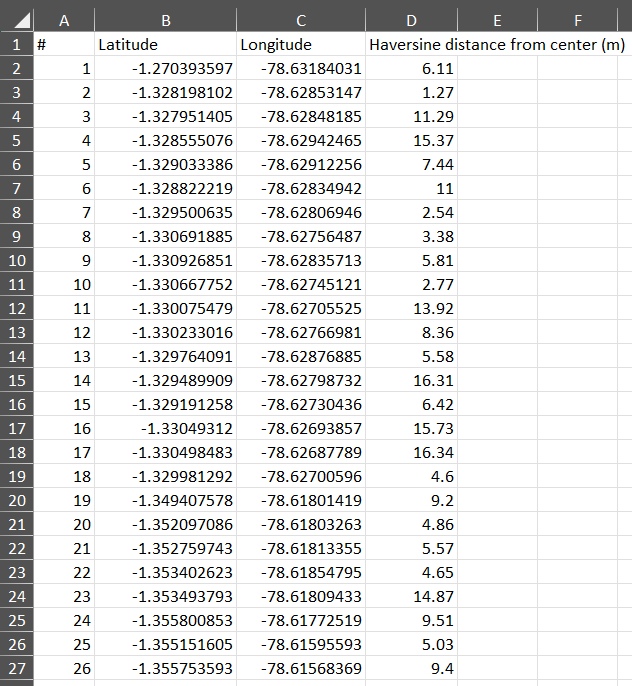
\includegraphics[width=0.5\textwidth]{chapters/III-resultados-y-discusion/resources/images/archivo-excel-georreferenciacion.png}
    \caption{Archivo de Excel con los datos georreferenciados para la comparación.}
    \label{fig:archivo-excel-georreferenciacion}
\end{figure}

Utilizando estos datos se creo un cluster de puntos georreferenciados en python, para ello se utilizó el algoritmo de K-Means, el cual
permite agrupar los puntos en clusters en función de su distancia. El código utilizado para la creación del cluster se muestra en la
Figura \ref{fig:script-cluster-python}. Utilizando el método del codo se determinó el número óptimo de clusters, el cual fue de 2 como
se muestra en la Figura \ref{fig:metodo-del-codo} en done se puede observar que el codo se encuentra en el punto 2.

\begin{figure}[H]
    \begin{minted}[fontsize=\footnotesize, linenos, breaklines, frame=single]{python}
import pandas as pd
import matplotlib.pyplot as plt
from sklearn.cluster import KMeans
import pygments as pg

df = pd.read_excel('geo-locations.xlsx', usecols='B:D', skiprows=0)
df.columns = ['latitude', 'longitude', 'distance']

# Elbow Method
def elbow_method(data):
    wcss = []
    for i in range(1, 11):
        kmeans = KMeans(n_clusters=i, max_iter=300)
        kmeans.fit(df[['latitude', 'longitude']])
        wcss.append(kmeans.inertia_)
    plt.plot(range(1, 11), wcss)
    plt.title('Método del Codo')
    plt.xlabel('Número de clusters')
    plt.ylabel('WCSS (Within Cluster Sum of Squares)')
    plt.show()

elbow_method(df)

# Cluster optimal number
numero_optimo_clusters = 2

# apply K-Means
kmeans = KMeans(n_clusters=numero_optimo_clusters, max_iter=300, random_state=42)
kmeans.fit(df[['latitude', 'longitude']])
df['cluster'] = kmeans.labels_

# Calc the mean distance of each cluster
distancias_medias_clusters = df.groupby('cluster')['distance'].mean()
print("Distancias medias de cada cluster:")
print(distancias_medias_clusters)

# Calc the mean of the mean distances of the clusters
media_de_las_medias = round(distancias_medias_clusters.mean(), 2)
print("Media de las distancias medias de los clusters:")
print(media_de_las_medias)

# Graph
plt.scatter(df['latitude'], df['longitude'], c=df['cluster'], cmap='viridis')
plt.title('Clusters de Puntos GPS')
plt.xlabel('Latitud')
plt.ylabel('Longitud')
plt.colorbar(label='Cluster')
plt.show()

\end{minted}


    \caption{Script en Python para la creación de clusters de puntos georreferenciados.}
    \label{fig:script-cluster-python}
\end{figure}

\begin{figure}[H]
    \centering
    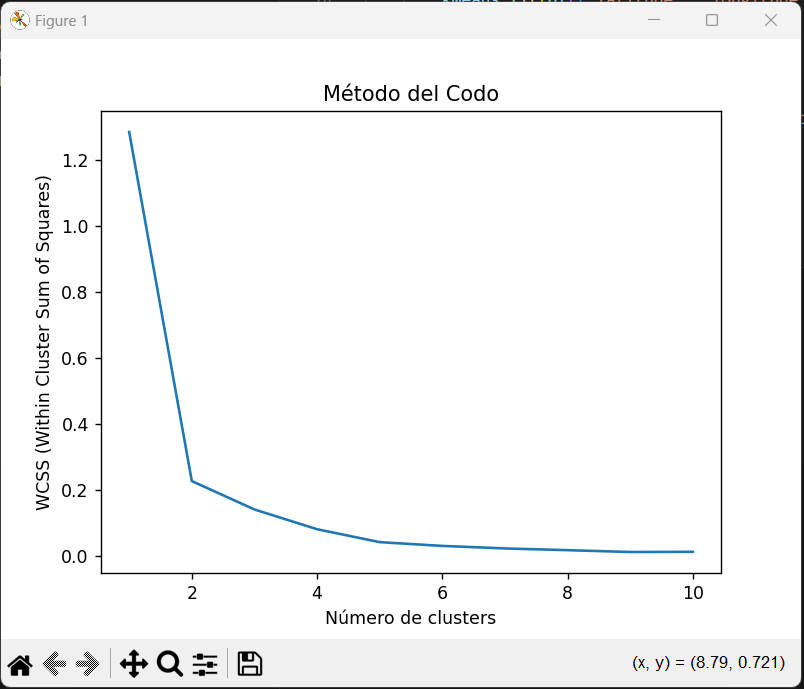
\includegraphics[width=0.5\textwidth]{chapters/III-resultados-y-discusion/resources/images/metodo-del-codo.png}
    \caption{Método del codo para determinar el número óptimo de clusters.}
    \label{fig:metodo-del-codo}
\end{figure}

El cluster resultante aplicando el algoritmo de K-Means se muestra en la Figura \ref{fig:cluster-georreferenciacion}.

\begin{figure}[H]
    \centering
    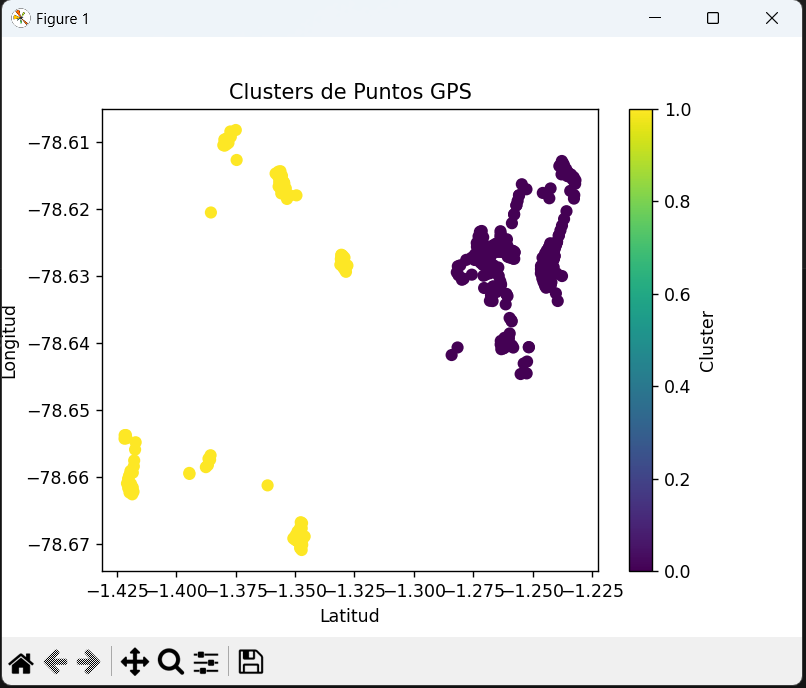
\includegraphics[width=0.5\textwidth]{chapters/III-resultados-y-discusion/resources/images/cluster-georreferenciacion.png}
    \caption{Cluster de puntos georreferenciados obtenidos mediante el algoritmo de K-Means.}
    \label{fig:cluster-georreferenciacion}
\end{figure}

Posteriormente se calculó la distancia media de cada cluster, así como la media de las distancias medias de los clusters. Los resultados
se muestran a continuación:

\begin{itemize}
    \item Distancias medias de cada cluster:
          \begin{itemize}
              \item Cluster 1: 6.32 m
              \item Cluster 2: 8.78 m
          \end{itemize}
    \item Media de las distancias medias de los clusters: 7.55 m
\end{itemize}

Estos resultados indican que la precisión media de los cluster es de 7.55 metros, Con la finalidad de obtener el intervalo de
confianza para esta media, se utilizó la Ecuación \ref{eq:ecuacion-intervalo-confianza}, donde:

\begin{itemize}
    \item IC = Intervalo de confianza
    \item M = Media de las distancias medias de los clusters
    \item ME = Margen de error
\end{itemize}

\begin{equation}
    IC = M \pm ME
    \label{eq:ecuacion-intervalo-confianza}
\end{equation}

El margen de error se calculó utilizando la Ecuación \ref{eq:ecuacion-margen-error}, donde:

\begin{itemize}
    \item ME = Margen de error
    \item Z = Valor crítico de la distribución normal estándar
    \item SE = Error estándar
\end{itemize}

\begin{equation}
    ME = Z \times SE
    \label{eq:ecuacion-margen-error}
\end{equation}

El error estándar se calculó utilizando la Ecuación \ref{eq:ecuacion-error-estandar}, donde:

\begin{itemize}
    \item SE = Error estándar
    \item $\sigma$ = Desviación estándar
    \item k = Tamaño de la muestra
\end{itemize}

\begin{equation}
    SE = \frac{\sigma}{\sqrt{k}}
    \label{eq:ecuacion-error-estandar}
\end{equation}


Sustituyendo los valores en las Ecuaciones \ref{eq:ecuacion-error-estandar} y \ref{eq:ecuacion-margen-error}, se obtiene:

\begin{itemize}
    \item Z = 1.96, con un nivel de confianza del 95\%
    \item $\sigma$ = 4.77
    \item k = 385
\end{itemize}

\begin{equation}
    SE = \frac{4.77}{\sqrt{385}} = 0.24
    \label{eq:ecuacion-resultado-error-estandar}
\end{equation}

\begin{equation}
    ME = 1.96 \times 0.24 = 0.47
    \label{eq:ecuacion-resultado-margen-error}
\end{equation}

Sustituyendo los valores en la Ecuación \ref{eq:ecuacion-intervalo-confianza} para el intervalo de confianza, se obtiene:

\begin{itemize}
    \item ME = 0.47
    \item M = 7.55
\end{itemize}

\begin{equation}
    IC = 7.55 \pm 0.47 = [7.08, 8.02]
    \label{eq:ecuacion-resultado-intervalo-confianza}
\end{equation}

Por lo tanto, se tiene que para un nivel de confianza del 95\%, el error de estimación de la precisión de los datos georreferenciados
se encuentra entre 7.08 y 8.02 metros con respecto al punto real de la ubicación.

\subsection{Desarrollo de la propuesta}
Para desarrollar la propuesta, se utilizó la metodología RAD, una metodología ágil para el desarrollo de software
creada por James Martin en 1991 \cite{agrawalUSINGRAPIDAPPLICATION2019}. Esta metodología se compone de las
siguientes cuatro fases:

\begin{enumerate}
    \item Planificación de requerimientos: En la fase de planificación de requerimientos, el usuario y el analista
          se reúnen para definir el objetivo de la aplicación o sistema y determinar los requisitos de información
          necesarios para alcanzar ese objetivo, el enfoque en esta etapa es resolver problemas empresariales \cite{maulanyDesignLearningApplications2021}.
    \item Diseño de usuario: El diseño de la aplicación se basará en esta descripción y será beneficioso para
          todos. La segunda fase de RAD implica la creación de diagramas ERD, UML y otros, así como el diseño de
          la interfaz de usuario mediante prototipos \cite{maulanyDesignLearningApplications2021}.
    \item Construcción: La etapa de construcción se enfoca en la programación y producción de código del sistema \cite{fauziSystematicLiteratureReviews2023}.
    \item Cierre: La etapa de cierre consiste en la puesta a prueba de la aplicación \cite{fauziSystematicLiteratureReviews2023}.
\end{enumerate}

\subsection{Planificación de requerimientos}
En esta fase, se identificaron los requerimientos del sistema a través de la recopilación de información de los
usuarios y las entrevistas realizadas.
\bigbreak

A continuación, en la tabla \ref{tab:descripcion-usuarios}, se describen los usuarios y la forma en que interactúan con
el sistema web y móvil.

\label{app:descripcion-usuarios}
\begin{longtable}{|p{3cm}|p{10cm}|}
    \caption{Descripción de usuarios} \label{tab:descripcion-usuarios}                                                                                                                                                                                               \\

    \hline \multicolumn{1}{|c|}{\textbf{Usuario}} & \multicolumn{1}{|c|}{\textbf{Descripción}}                                                                                                                                                                       \\ \hline
    \endfirsthead

    \multicolumn{2}{c}%
    {{\normalfont \tablename\ \thetable{} -- continuación de la página anterior}}                                                                                                                                                                                    \\
    \hline \multicolumn{1}{|c|}{\textbf{Usuario}} & \multicolumn{1}{|c|}{\textbf{Descripción}}                                                                                                                                                                       \\ \hline
    \endhead

    \hline \multicolumn{2}{|r|}{{Continua en la siguiente página}}                                                                                                                                                                                                   \\ \hline
    \endfoot

    \hline \hline
    \endlastfoot
    Administrador del sistema                     &
    Usuario responsable de gestionar a otros usuarios, las zonas de vigilancia y los tipos de delitos, además de monitorear los incidentes delictivos, coordinar el despacho de las entidades correspondientes y tomar decisiones basadas en los reportes generados. \\\hline
    Usuario ciudadano                             & Usuario encargado de enviar alertas sobre incidentes delictivos.                                                                                                                                                 \\\hline
    Policía                                       & Usuario encargado de recibir y atender las alertas de incidentes delictivos.                                                                                                                                     \\
\end{longtable}

En la tabla \ref{tab:requerimientos} se presentan los requerimientos definidos para el desarrollo del proyecto.

\newcounter{reqcounter}
\setcounter{reqcounter}{1}

\begin{longtable}{|p{0.6cm}|p{3cm}|p{6.3cm}|c|c|}
    \caption{Definición de requerimientos} \label{tab:requerimientos}                                                                                                                                                                                                                                                                   \\

    \hline \multicolumn{1}{|c|}{\textbf{ID}}     & \multicolumn{1}{|c|}{\textbf{Requerimiento}}       & \multicolumn{1}{|c|}{\textbf{Descripción}}                                                                                                   & \multicolumn{1}{|c|}{\textbf{Prioridad}} & \multicolumn{1}{|c|}{\textbf{Riesgo}} \\ \hline
    \endfirsthead

    \multicolumn{5}{c}%
    {{\normalfont \tablename\ \thetable{} -- continuación de la página anterior}}                                                                                                                                                                                                                                                       \\
    \hline \multicolumn{1}{|c|}{\textbf{ID}}     & \multicolumn{1}{|c|}{\textbf{Requerimiento}}       & \multicolumn{1}{|c|}{\textbf{Descripción}}                                                                                                   & \multicolumn{1}{|c|}{\textbf{Prioridad}} & \multicolumn{1}{|c|}{\textbf{Riesgo}} \\ \hline
    \endhead

    \hline
    \multicolumn{5}{|c|}{{Continua en la siguiente página}}                                                                                                                                                                                                                                                                             \\
    \hline
    \endfoot

    \hline
    \endlastfoot

    \multicolumn{5}{|l|}{\textbf{Todos los usuarios de la aplicación web y móvil}}                                                                                                                                                                                                                                                      \\
    \hline
    R\arabic{reqcounter}\stepcounter{reqcounter} & Iniciar Sesión                                     & El inicio de sesión se realizará a través de la autenticación del usuario, quien deberá ingresar su correo y contraseña.                     & Alta                                     & Alto                                  \\
    \hline
    R\arabic{reqcounter}\stepcounter{reqcounter} & Cerrar Sesión                                      & El usuario podrá cerrar la sesión en cualquier momento.                                                                                      & Alta                                     & Bajo                                  \\
    \hline
    \multicolumn{5}{|l|}{\textbf{Administrador del sistema}}                                                                                                                                                                                                                                                                            \\
    \hline
    R\arabic{reqcounter}\stepcounter{reqcounter} & Administrar usuarios                               & El adminsitrador podrá crear, visualizar, actualizar y deshabilitar usuarios                                                                 & Alta                                     & Alto                                  \\
    \hline
    R\arabic{reqcounter}\stepcounter{reqcounter} & Gestionar tipos de incidentes                      & El administrador podrá crear, visualizar, actualizar y deshabilitar tipos de incidentes                                                      & Alta                                     & Alto                                  \\
    \hline
    R\arabic{reqcounter}\stepcounter{reqcounter} & Gestionar zonas de vigilancia                      & El administrador podrá crear, visualizar, actualizar y deshabilitar tipos de incidentes                                                      & Alta                                     & Alto                                  \\
    \hline
    R\arabic{reqcounter}\stepcounter{reqcounter} & Asignar policías a las zonas de vigilancia         & El administrador podra asignar y desasignar miembros de la policias a las zonas de vigilancia                                                & Alta                                     & Alto                                  \\
    \hline
    R\arabic{reqcounter}\stepcounter{reqcounter} & Visualizar alertas de incidentes                   & El administrador podrá visualizar mediante un mapa las alertas de emergencia enviadas por los ciudadanas asi como su posición en tiempo real & Alta                                     & Alto                                  \\
    \hline
    R\arabic{reqcounter}\stepcounter{reqcounter} & Visualizar mapas de calor                          & El administrador podrá visualizar mediante un mapa de calor los incidentes delictivos suscitados en las diferentes zonas                     & Alta                                     & Bajo                                  \\
    \hline
    R\arabic{reqcounter}\stepcounter{reqcounter} & Visualizar reportes                                & El administrador podrá visualizar informes detallados sobre los incidentes ocurridos, generados mediante BI.                                 & Alta                                     & Alto                                  \\
    \hline
    \multicolumn{5}{|l|}{\textbf{Usuario ciudadano}}                                                                                                                                                                                                                                                                                    \\
    \hline
    R\arabic{reqcounter}\stepcounter{reqcounter} & Registro de usuario                                & Los usuarios deberán ingresar sus datos y fotografía mediante un formulario.                                                                 & Alta                                     & Alto                                  \\
    \hline
    R\arabic{reqcounter}\stepcounter{reqcounter} & Cambiar contraseña                                 & El usuario podrá cambiar su contraseña en cualquier momento.                                                                                 & Media                                    & Alto                                  \\
    \hline
    R\arabic{reqcounter}\stepcounter{reqcounter} & Recuperar contraseña                               & El usuario podrá recuperar su contraseña en caso de olvidarla mediante su correo electrónico.                                                & Baja                                     & Alto                                  \\
    \hline
    R\arabic{reqcounter}\stepcounter{reqcounter} & Asignar miembros a su grupo familiar               & El usuario podrá asignar miembros a su grupo familiar mediante la cédula de ciudadania.                                                      & Alta                                     & Alto                                  \\
    \hline
    R\arabic{reqcounter}\stepcounter{reqcounter} & Enviar alertas de emergencia                       & El usuario podrá enviar alertas de emergencia seleccionando el tipo de incidente y oprimiendo un botón de panica durante 3 segundos.         & Alta                                     & Alto                                  \\
    \hline
    R\arabic{reqcounter}\stepcounter{reqcounter} & Visualizar alertas de emergencia de familiares     & El usuario podrá visualizar mediante un mapa las alertas de emergencia enviadas por los sus familiares asi como su posición en tiempo real.  & Alta                                     & Alto                                  \\
    \hline
    \multicolumn{5}{|l|}{\textbf{Policía}}                                                                                                                                                                                                                                                                                              \\
    \hline
    R\arabic{reqcounter}\stepcounter{reqcounter} & Visualizar alertas de emergencia de los ciudadanos & El policía podrá visualizar mediante un mapa las alertas de emergencia enviadas por los ciudadanas asi como su posición en tiempo real       & Alta                                     & Alto                                  \\
    \hline
\end{longtable}

Una vez definidos los requerimientos necesarios, se elaboró el siguiente plan de iteraciones para estructurar y gestionar
el desarrollo del proyecto.

\newcounter{numcounter}
\newcounter{itcounter}
\setcounter{numcounter}{1}
\setcounter{itcounter}{1}
\setcounter{reqcounter}{1}

\begin{longtable}{|p{0.6cm}|p{0.6cm}|p{0.6cm}|p{3cm}|c|c|}
    \caption{Planificación de iteraciones} \label{tab:planificacion-iteraciones}                                                                                                                                                                                                                                        \\

    \hline \multicolumn{1}{|c|}{\textbf{Iteración}}                      & \multicolumn{1}{|c|}{\textbf{N.}}           & \multicolumn{1}{|c|}{\textbf{ID}}            & \multicolumn{1}{|c|}{\textbf{Requerimientos}}      & \multicolumn{1}{|c|}{\textbf{Tiempo horas}} & \multicolumn{1}{|c|}{\textbf{Estimado días}} \\ \hline
    \endfirsthead

    \multicolumn{6}{c}%
    {{\normalfont \tablename\ \thetable{} -- continuación de la página anterior}}                                                                                                                                                                                                                                       \\
    \hline \multicolumn{1}{|c|}{\textbf{Iteración}}                      & \multicolumn{1}{|c|}{\textbf{N.}}           & \multicolumn{1}{|c|}{\textbf{ID}}            & \multicolumn{1}{|c|}{\textbf{Requerimientos}}      & \multicolumn{1}{|c|}{\textbf{Tiempo horas}} & \multicolumn{1}{|c|}{\textbf{Estimado días}} \\ \hline
    \endhead

    \hline \multicolumn{6}{|r|}{{Continua en la siguiente página}}                                                                                                                                                                                                                                                      \\ \hline
    \endfoot

    \hline \hline
    \endlastfoot
    \multirow{4}{*}{Iteración \arabic{itcounter}\stepcounter{itcounter}} & \arabic{numcounter}\stepcounter{numcounter} & R\arabic{reqcounter}\stepcounter{reqcounter} & Iniciar sesión                                     & 6                                           & 1                                            \\\cline{2-6}
                                                                         & \arabic{numcounter}\stepcounter{numcounter} & R\arabic{reqcounter}\stepcounter{reqcounter} & Cerrar sesión                                      & 1                                           & 1                                            \\\cline{2-6}
                                                                         & \arabic{numcounter}\stepcounter{numcounter} & R\arabic{reqcounter}\stepcounter{reqcounter} & Registro de usuario                                & 12                                          & 2                                            \\\cline{2-6}
                                                                         & \arabic{numcounter}\stepcounter{numcounter} & R\arabic{reqcounter}\stepcounter{reqcounter} & Cambiar contraseña                                 & 2                                           & 1                                            \\\cline{2-6}
                                                                         & \arabic{numcounter}\stepcounter{numcounter} & R\arabic{reqcounter}\stepcounter{reqcounter} & Recuperar contraseña                               & 6                                           & 1                                            \\\hline
    \multirow{4}{*}{Iteración \arabic{itcounter}\stepcounter{itcounter}} & \arabic{numcounter}\stepcounter{numcounter} & R\arabic{reqcounter}\stepcounter{reqcounter} & Asignar miembros al grupo familiar                 & 6                                           & 1                                            \\\cline{2-6}
                                                                         & \arabic{numcounter}\stepcounter{numcounter} & R\arabic{reqcounter}\stepcounter{reqcounter} & Enviar alertas de emergencia                       & 18                                          & 3                                            \\\cline{2-6}
                                                                         & \arabic{numcounter}\stepcounter{numcounter} & R\arabic{reqcounter}\stepcounter{reqcounter} & Visualizar alertas de emergencia de familiares     & 12                                          & 2                                            \\\cline{2-6}
                                                                         & \arabic{numcounter}\stepcounter{numcounter} & R\arabic{reqcounter}\stepcounter{reqcounter} & Gestionar usuarios                                 & 6                                           & 1                                            \\\cline{2-6}
                                                                         & \arabic{numcounter}\stepcounter{numcounter} & R\arabic{reqcounter}\stepcounter{reqcounter} & Gestionar tipos de incidentes                      & 4                                           & 1                                            \\\hline
    \multirow{6}{*}{Iteración \arabic{itcounter}\stepcounter{itcounter}} & \arabic{numcounter}\stepcounter{numcounter} & R\arabic{reqcounter}\stepcounter{reqcounter} & Gestionar zonas de vigilancia                      & 18                                          & 3                                            \\\cline{2-6}
                                                                         & \arabic{numcounter}\stepcounter{numcounter} & R\arabic{reqcounter}\stepcounter{reqcounter} & Asignar policías a las zonas de vigilancia         & 5                                           & 1                                            \\\cline{2-6}
                                                                         & \arabic{numcounter}\stepcounter{numcounter} & R\arabic{reqcounter}\stepcounter{reqcounter} & Gestionar alertas de incidentes                    & 18                                          & 3                                            \\\cline{2-6}
                                                                         & \arabic{numcounter}\stepcounter{numcounter} & R\arabic{reqcounter}\stepcounter{reqcounter} & Visualizar mapa de calor                           & 6                                           & 1                                            \\\cline{2-6}
                                                                         & \arabic{numcounter}\stepcounter{numcounter} & R\arabic{reqcounter}\stepcounter{reqcounter} & Visualizar reportes                                & 84                                          & 14                                           \\\cline{2-6}
                                                                         & \arabic{numcounter}\stepcounter{numcounter} & R\arabic{reqcounter}\stepcounter{reqcounter} & Visualizar alertas de emergencia de los ciudadanos & 12                                          & 2                                            \\
\end{longtable}

\subsection{Diseño de usuario}

\subsubsection{Análisis del proceso propuesto}

En la Figura \ref{fig:proceso-propuesto} se presenta el proceso propuesto para el envió de alertas de emergencia con
ubicación en tiempo real, en donde:

\begin{enumerate}
    \item Si el usuario no se encuentra registrado en el sistema:
          \begin{enumerate}
              \item El usuario se registra en el sistema.
              \item El usuario inicia sesión en el sistema.
          \end{enumerate}
    \item El usuario ingresa miembros a su grupo familiar.
    \item El usuario selecciona un tipo de incidente.
          % \item El usuario envía la alerta de emergencia presionando el bot��������n de pánico durante 3 segundos.
    \item El usuario envía la alerta de emergencia presionando el botón de pánico durante 3 segundos.
    \item Se envía una notificación a los miembros del grupo familiar del usuario y los policías dentro de la zona de emergencia junto con la ubicación en tiempo real.
    \item El Ecu 911 recibe la alerta de emergencia y la asigna a la entidad correspondiente.
    \item La emergencia es atendida.
\end{enumerate}

\begin{figure}[H]
    \centering
    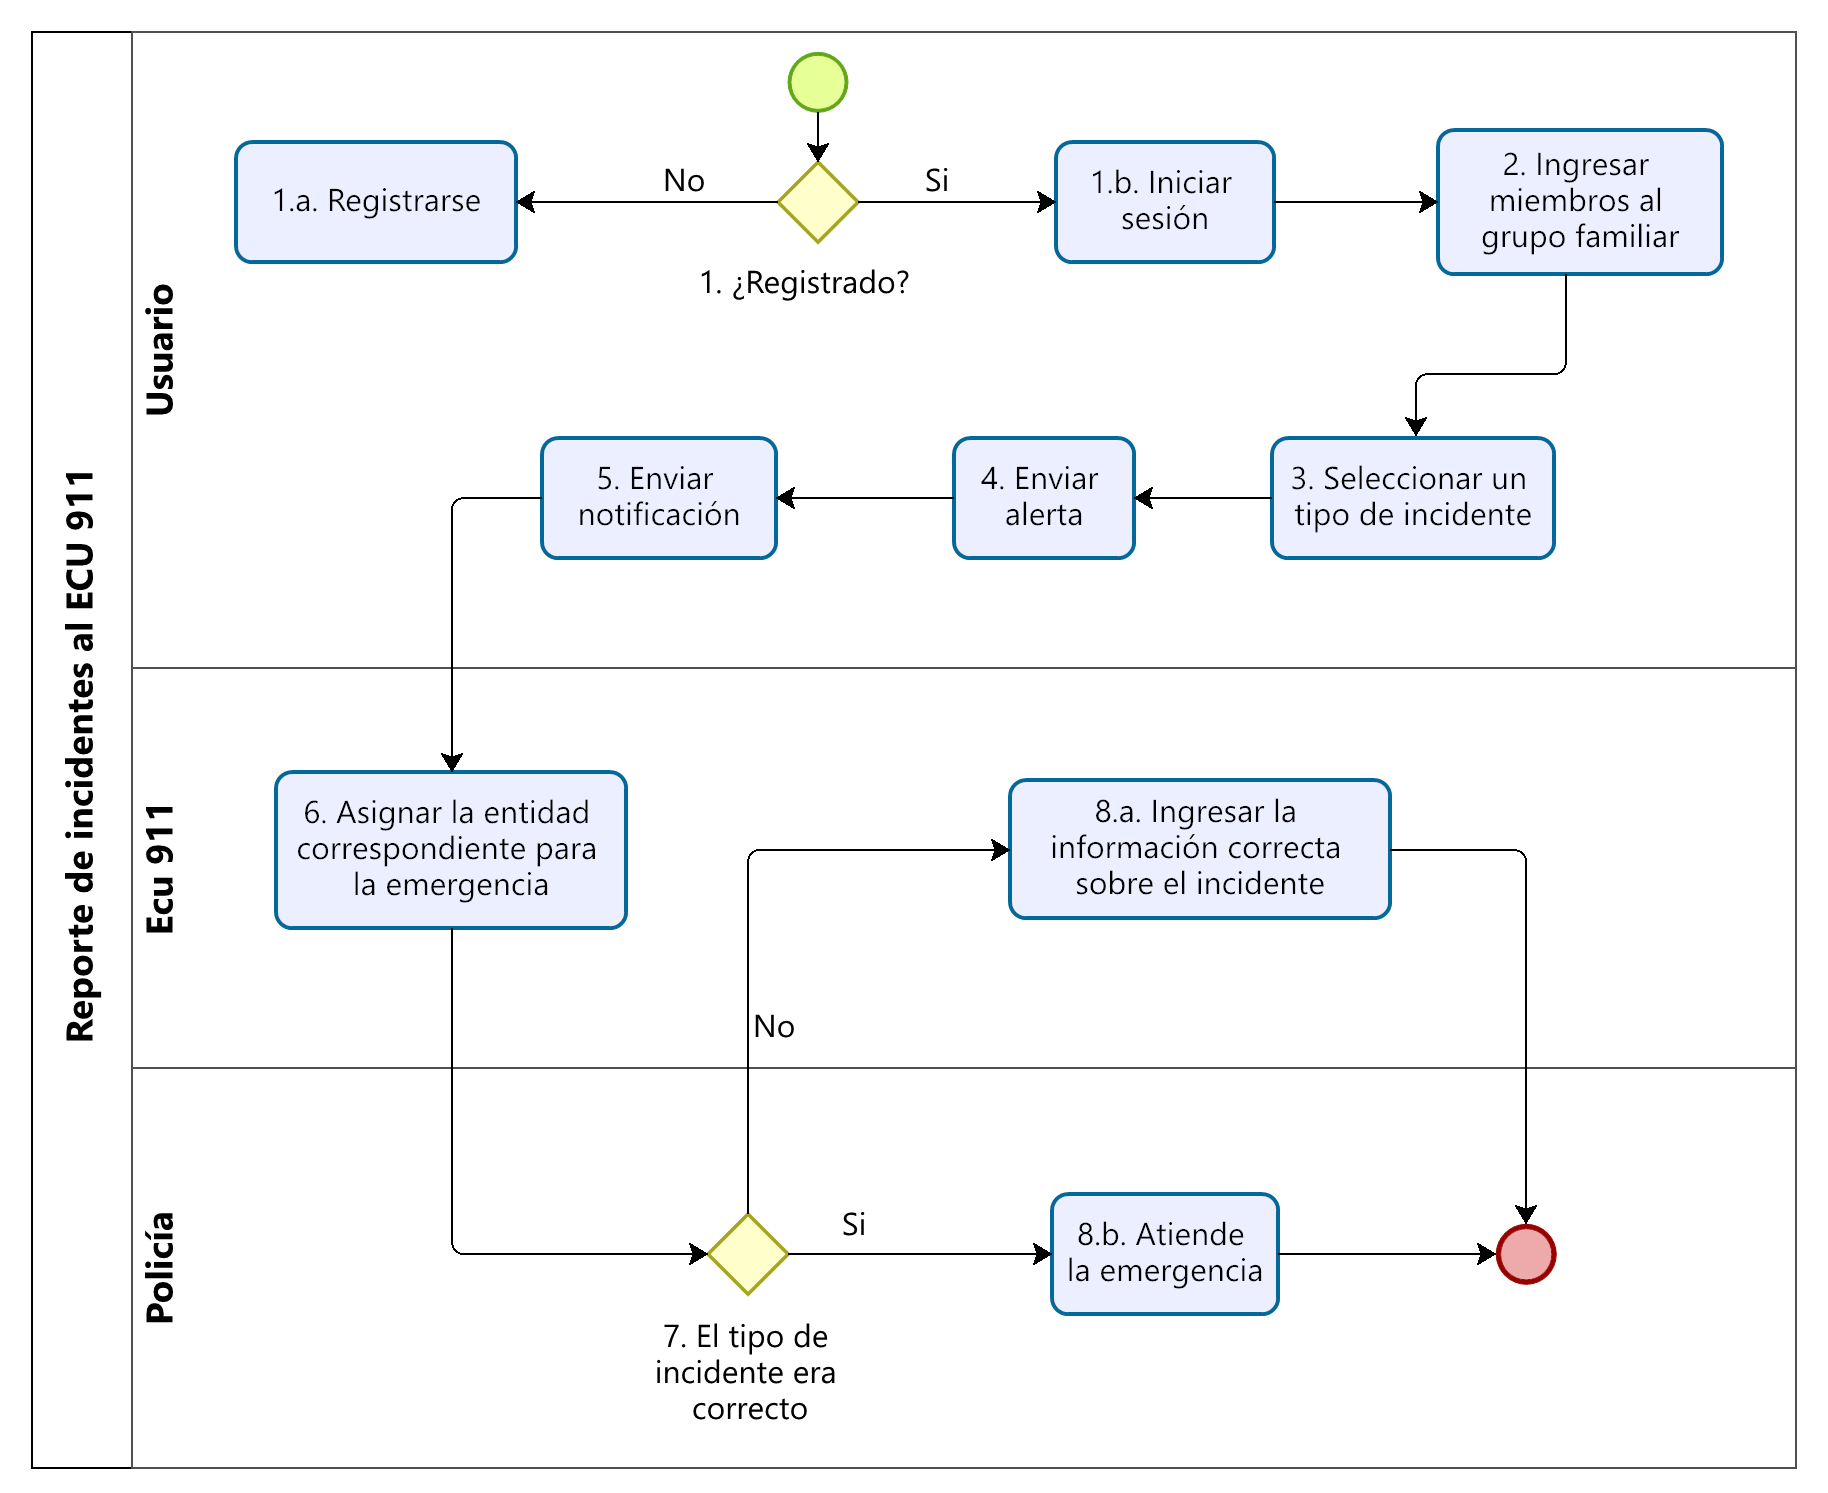
\includegraphics[width=0.8\textwidth]{chapters/III-resultados-y-discusion/resources/images/proceso-propuesto.png}
    \caption{Proceso propuesto de reporte de incidentes al ECU 911.}
    \label{fig:proceso-propuesto}
\end{figure}

\subsubsection{Arquitectura}

El desarrollo del sistema se estructuró en 2 partes fundamentales: la API y La interfaz de usuario, tanto web como móvil.
La interfaz de usuario en el sistema web permite a los administradores gestionar la información de los usuarios y los incidentes
ademas de visualizar la ubicación en tiempo real de los incidentes en un mapa. La interfaz de usuario en el sistema móvil
permite gestionar grupos familiares, enviar alertas de emergencia y visualizar la ubicación en tiempo real de los incidentes de sus
miembros del grupo familiar. El API se encuentra alojada en un servidor web y se encarga de gestionar la conexión entre la base de
datos, los servicios de almacenamiento de información, el servicio de hosting de imágenes, el servicio de web socket y las interfaces
de usuario.

\begin{figure}[H]
    \centering
    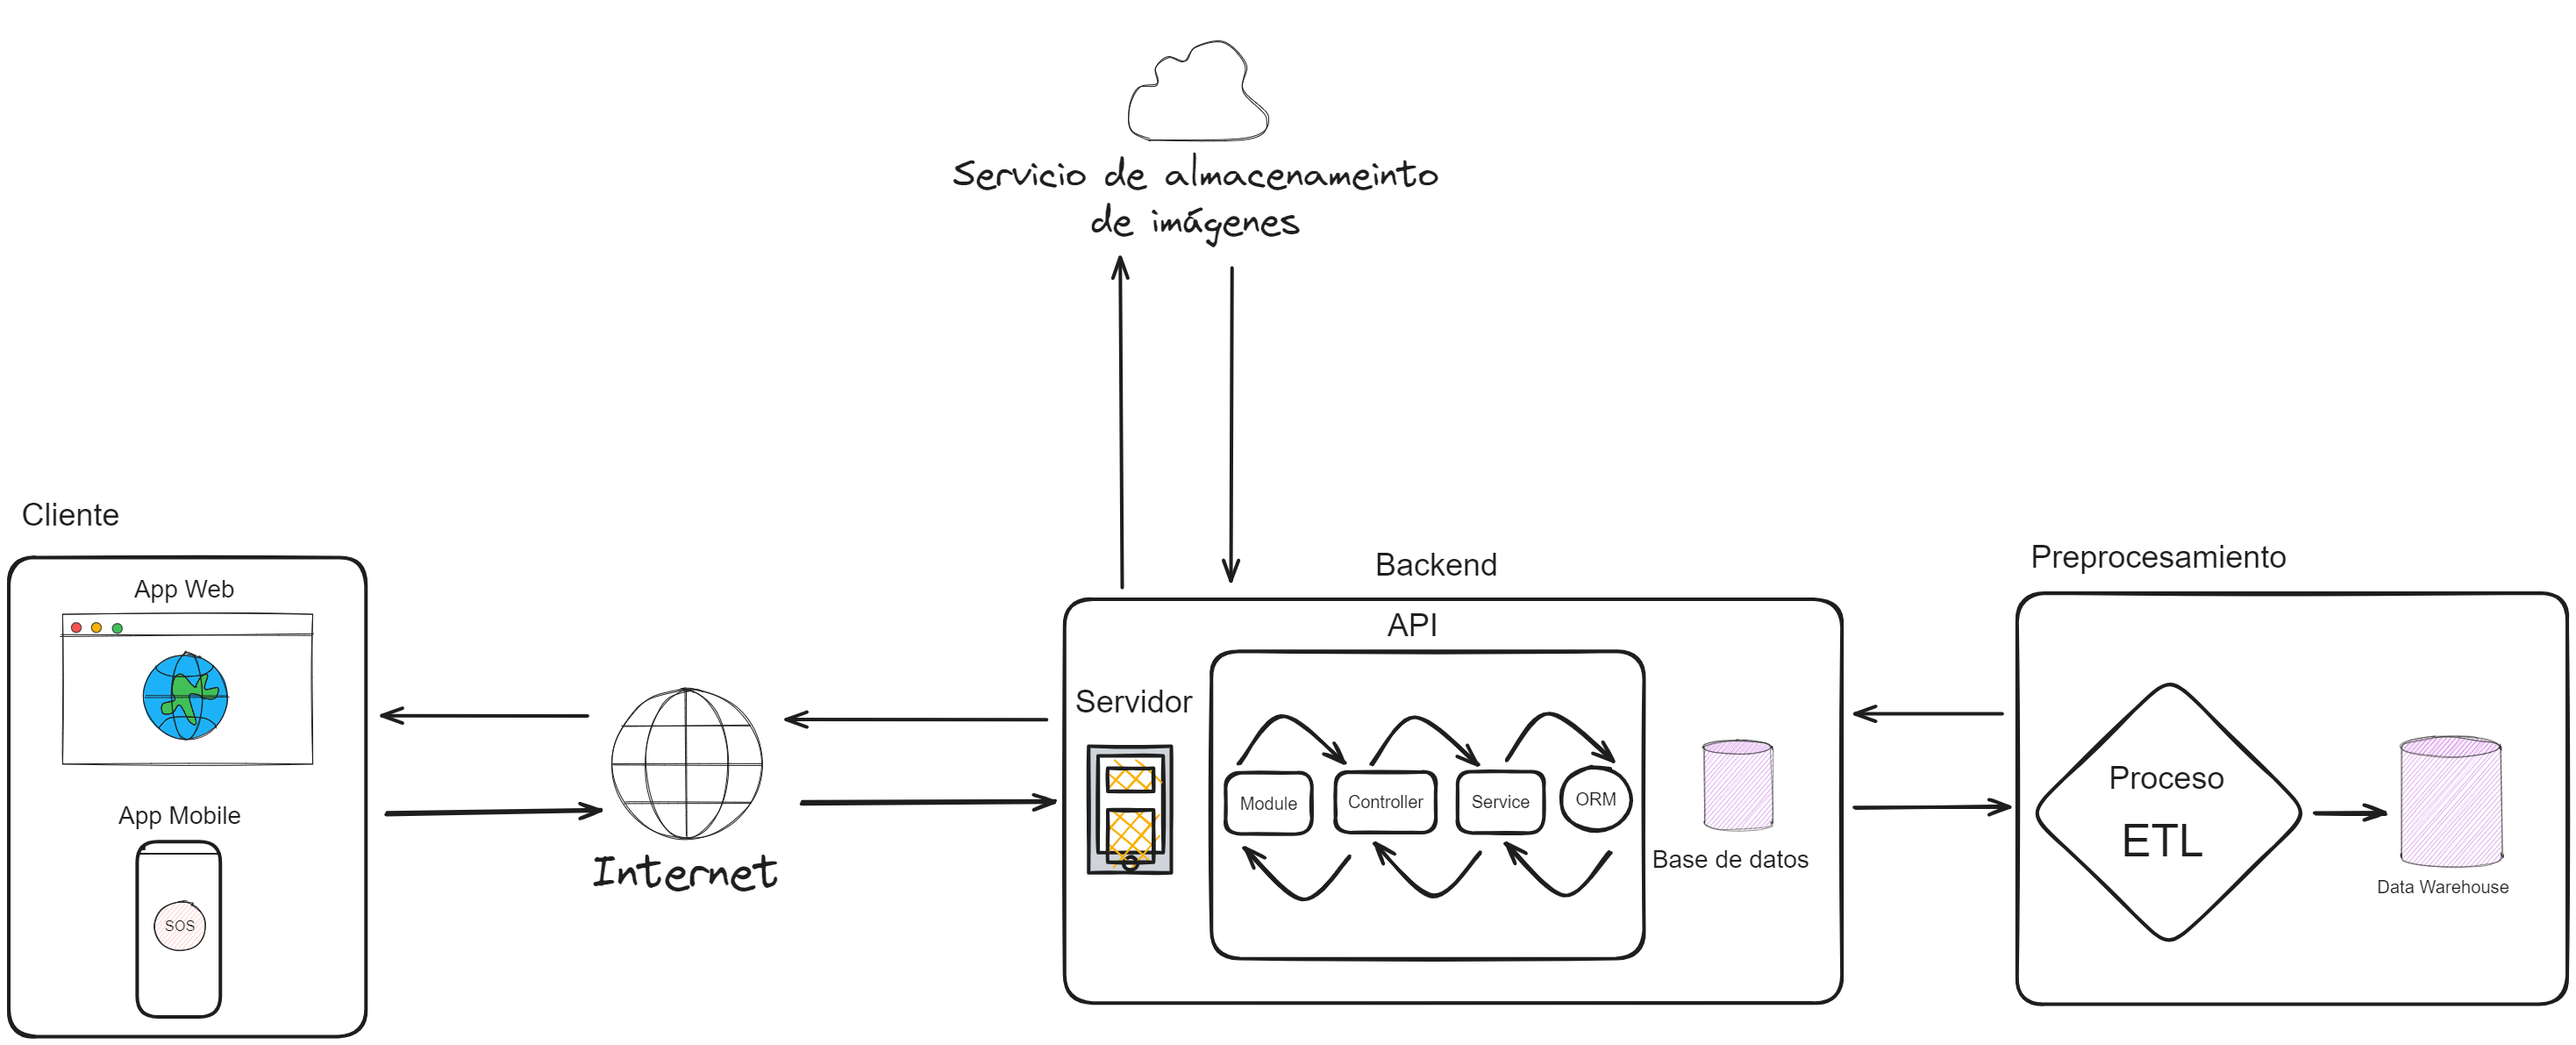
\includegraphics[width=1.1\textwidth]{chapters/III-resultados-y-discusion/resources/images/arquitectura.png}
    \caption{Arquitectura del sistema}
    \label{fig:arquitectura}
\end{figure}


\subsubsection{Prototipado}

En esta etapa de la metodología, se desarrollaron prototipos con el objetivo de identificar y resolver problemas de diseño y funcionalidad.
Esto permite detectar posibles fallos o áreas de mejora antes de la fase de construcción de la aplicación, optimizando así el proceso de
desarrollo y asegurando que el producto final sea más robusto y alineado con los objetivos del proyecto.

El prototipado para el sistema se divide en dos partes: el prototipo de la interfaz de usuario web y el prototipo de la interfaz de usuario móvil.

\subsubsection{Prototipo de la interfaz de usuario web}

En la Figura \ref{fig:prototipo-inicio-sesion-web} se presenta el prototipo de la interfaz de usuario web, donde se muestra la pantalla de inicio de sesión,
el cual se realiza mediante correo y contraseña.

\begin{figure}[H]
    \centering
    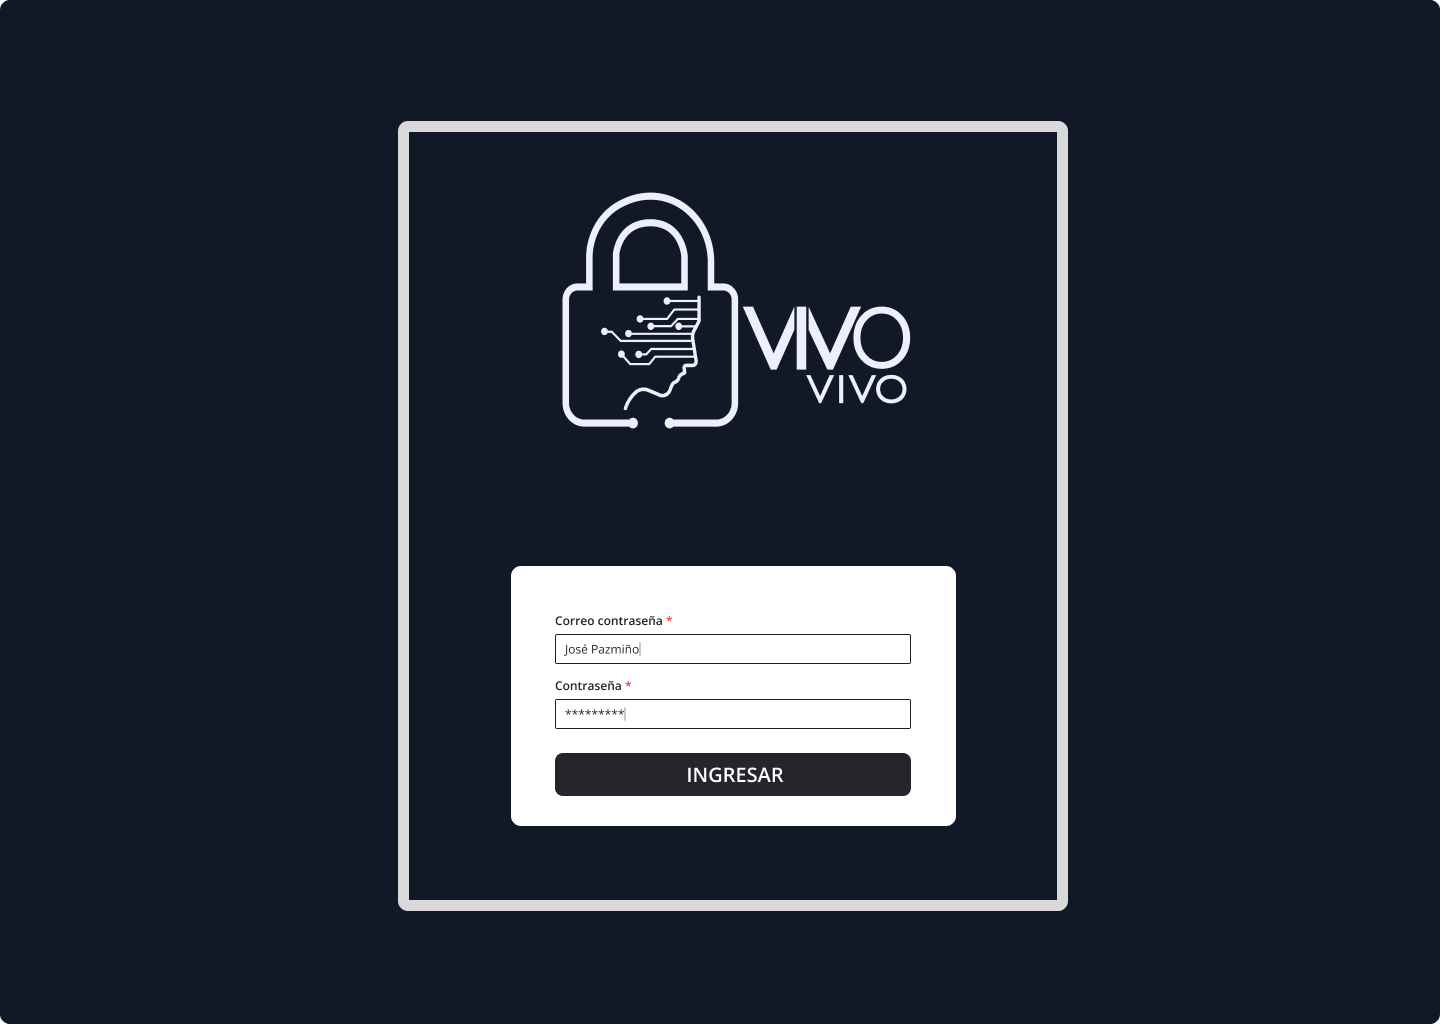
\includegraphics[width=0.6\textwidth]{chapters/III-resultados-y-discusion/resources/images/prototipo-inicio-sesion-web.png}
    \caption{Prototipo de la interfaz de usuario web: Inicio de sesión.}
    \label{fig:prototipo-inicio-sesion-web}
\end{figure}

En la Figura \ref{fig:prototipo-layout-web} se presenta el prototipo de la interfaz de usuario web, donde se muestra el layout de la aplicación web junto
con el menú de navegación y el menú de opciones

\begin{figure}[H]
    \centering
    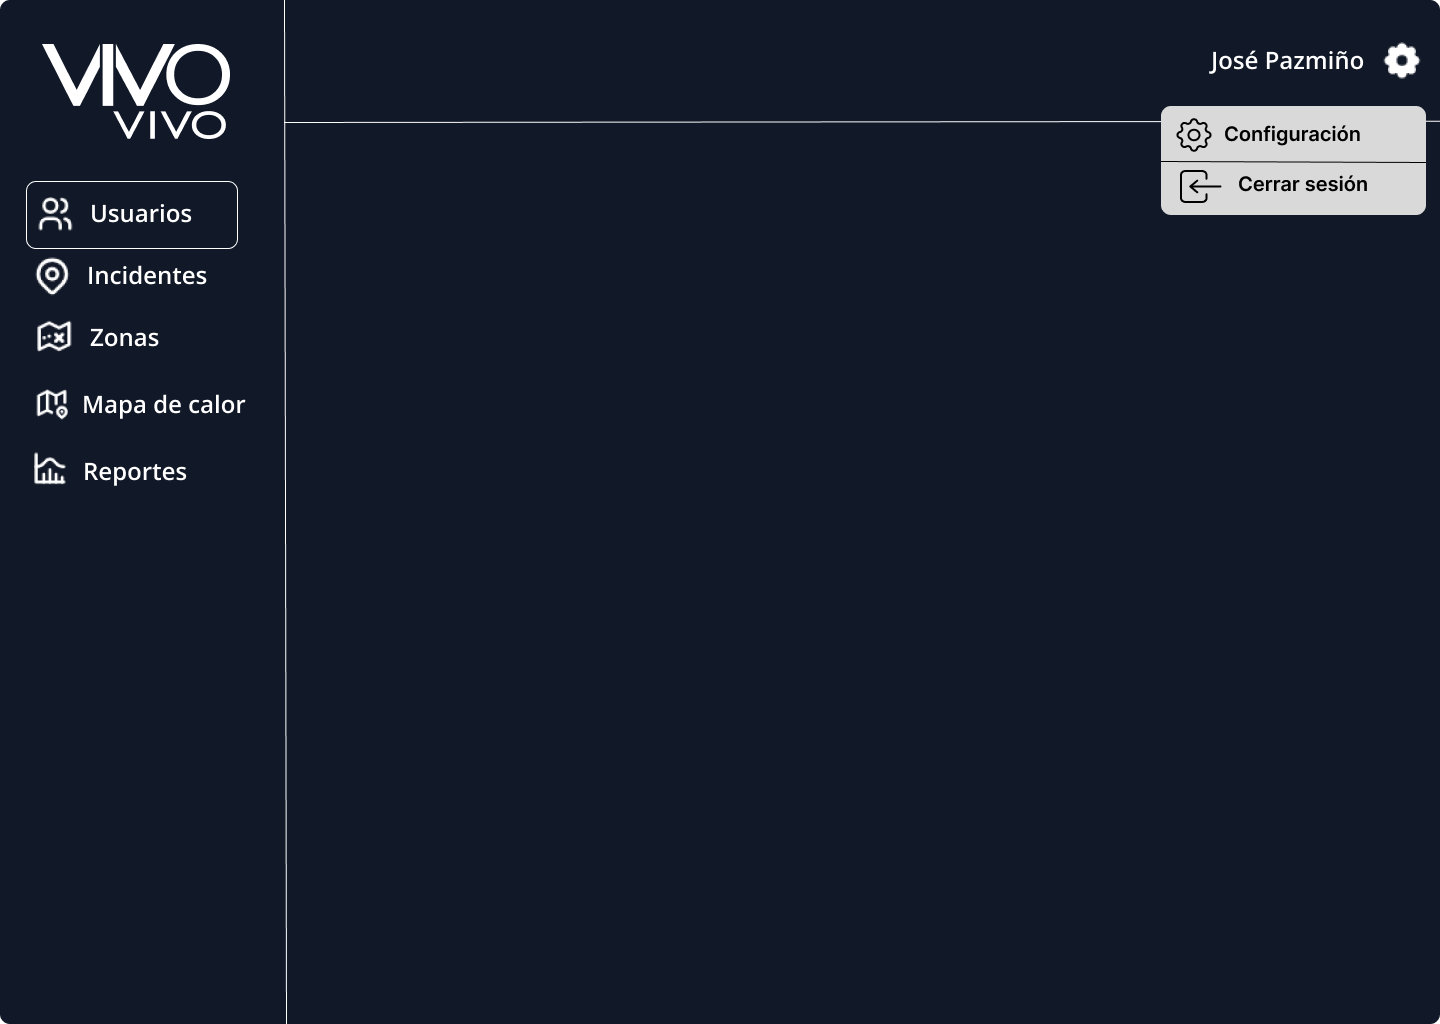
\includegraphics[width=0.6\textwidth]{chapters/III-resultados-y-discusion/resources/images/prototipo-layout-web.png}
    \caption{Prototipo de la interfaz de usuario web: Layout.}
    \label{fig:prototipo-layout-web}
\end{figure}

La gestión de la información en el sistema web se realiza a través de una tabla de entradas, la cual permite al usuario administrador crear, visualizar,
editar y eliminar los registros, así como también aplicar filtros de búsqueda, como se muestra en la Figura \ref{fig:prototipo-tabla-entradas-web}.

\begin{figure}[H]
    \centering
    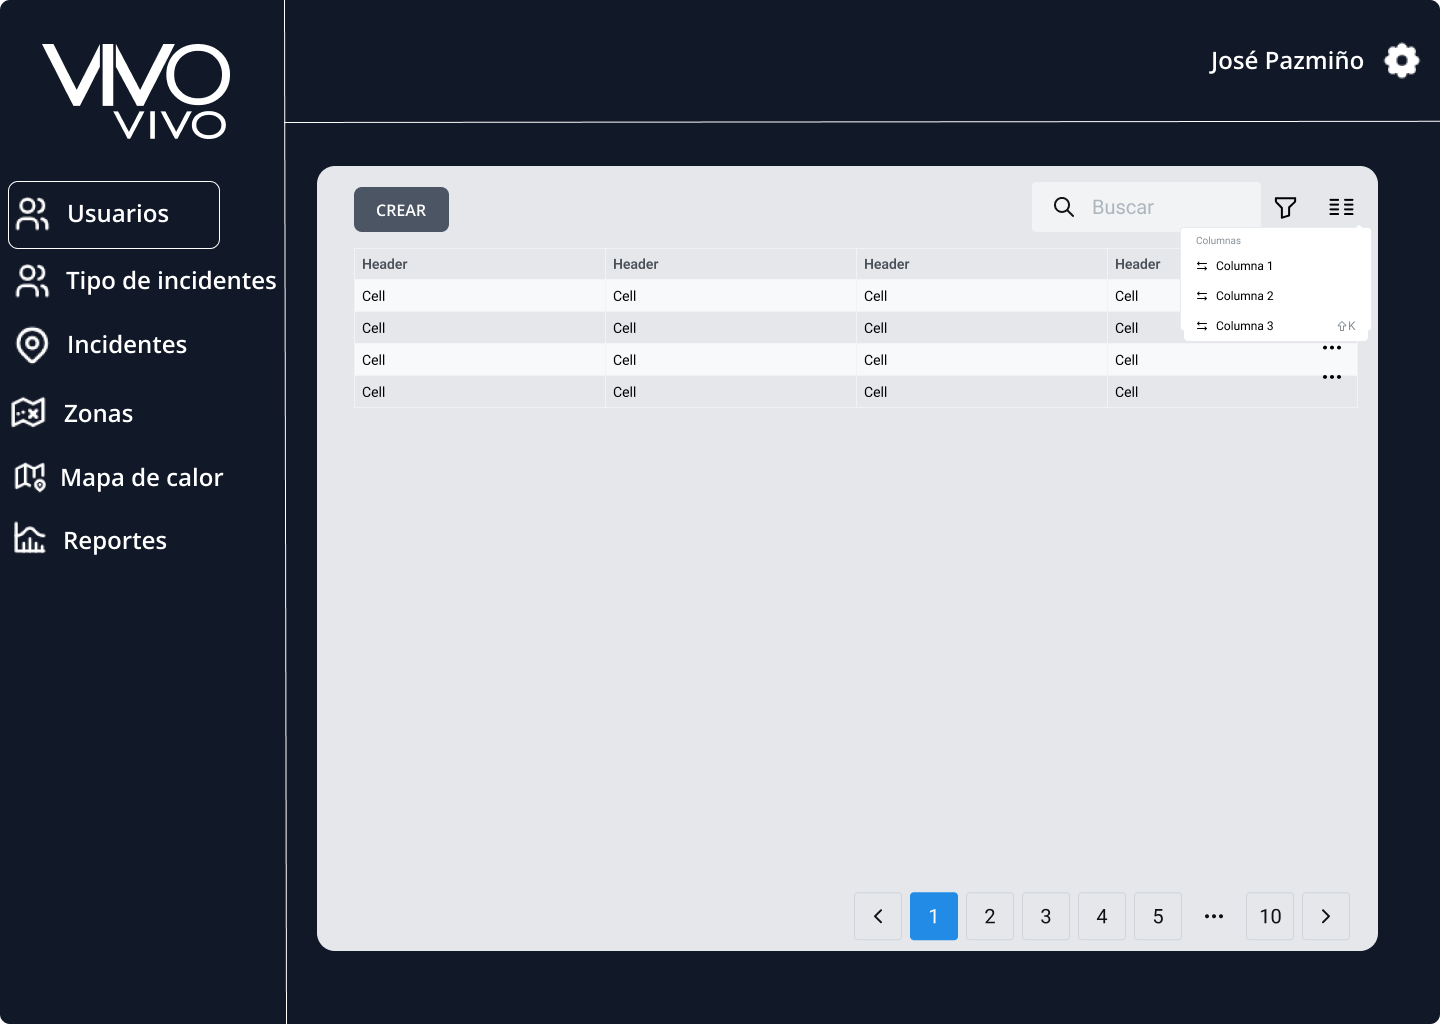
\includegraphics[width=0.6\textwidth]{chapters/III-resultados-y-discusion/resources/images/prototipo-tabla-entradas-web.png}
    \caption{Prototipo de la interfaz de usuario web: Tabla de entradas.}
    \label{fig:prototipo-tabla-entradas-web}
\end{figure}

En la Figura \ref{fig:prototipo-menu-tabla-entradas-web} se muestra el menú de opciones de la tabla de entradas, el cual permite al usuario administrador
realizar acciones como editar y eliminar registros. Al eliminar un registro, se muestra un mensaje de confirmación para ejecutar la acción, como se puede
observar en la Figura \ref{fig:prototipo-mensaje-eliminar-web}

\begin{figure}[H]
    \centering
    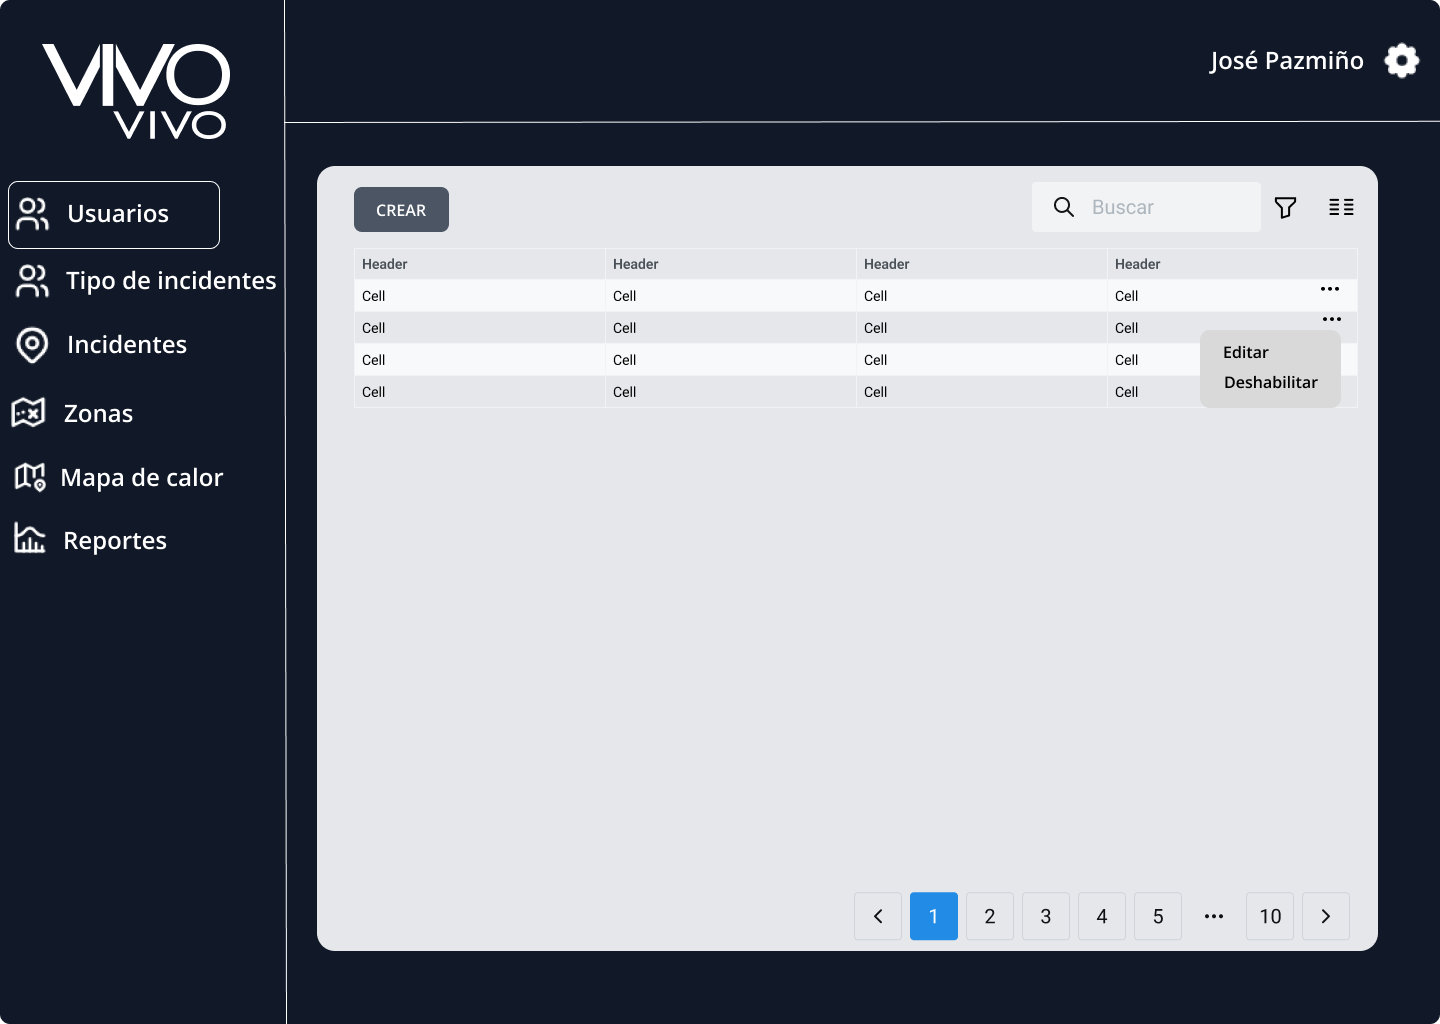
\includegraphics[width=0.6\textwidth]{chapters/III-resultados-y-discusion/resources/images/prototipo-menu-tabla-entradas-web.png}
    \caption{Prototipo de la interfaz de usuario web: Menú de opciones de la tabla de entradas.}
    \label{fig:prototipo-menu-tabla-entradas-web}
\end{figure}

\begin{figure}[H]
    \centering
    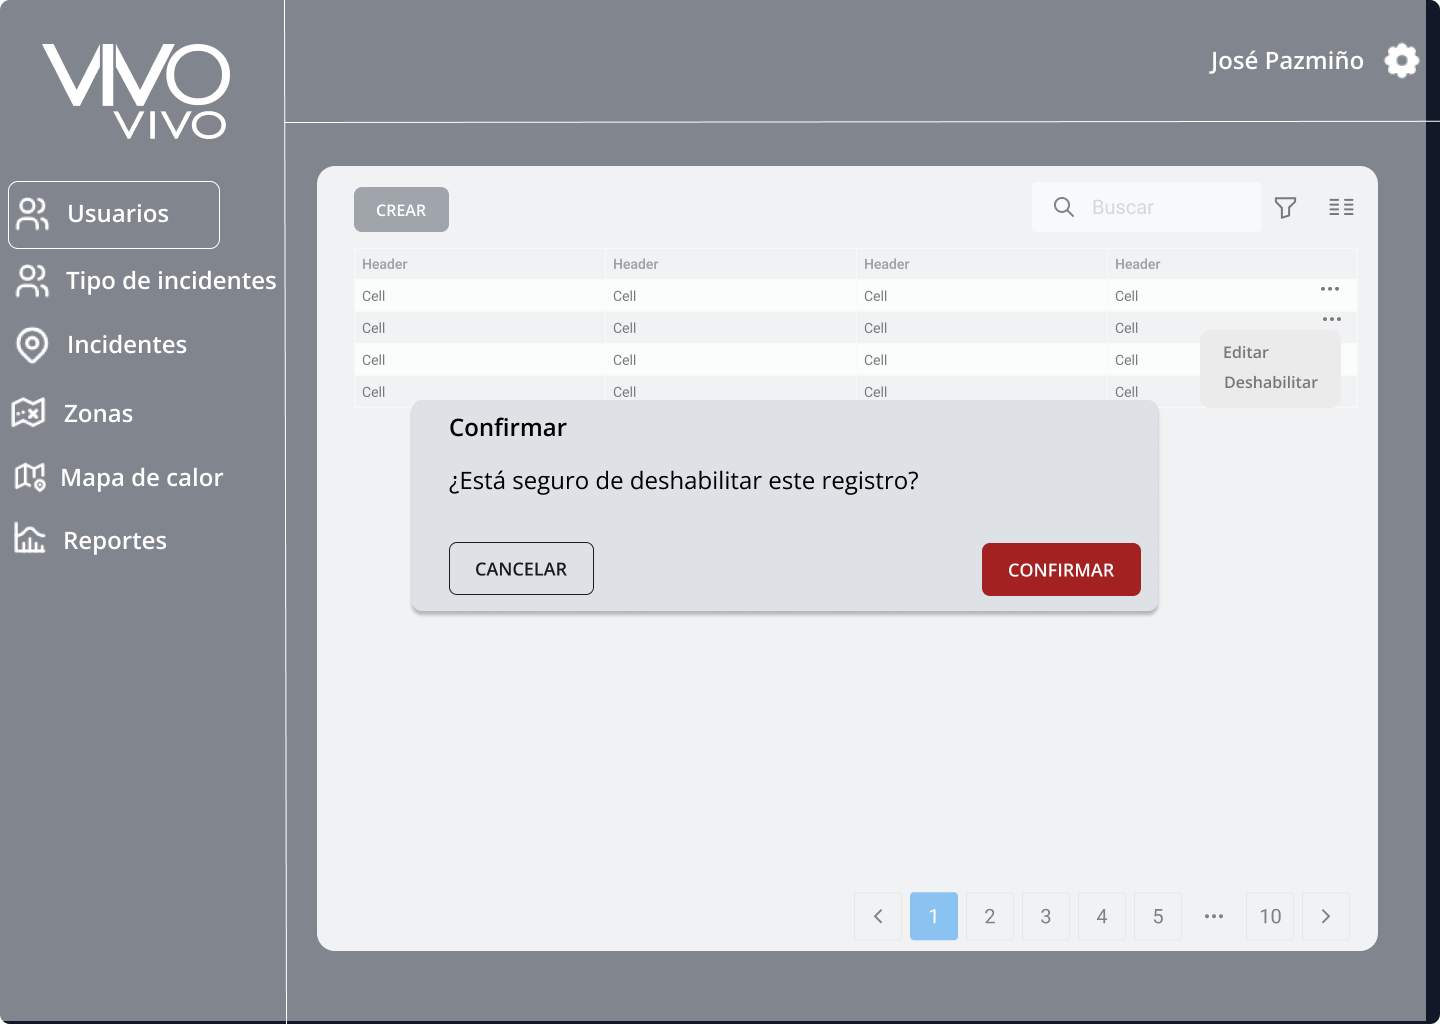
\includegraphics[width=0.6\textwidth]{chapters/III-resultados-y-discusion/resources/images/prototipo-mensaje-eliminar-web.png}
    \caption{Prototipo de la interfaz de usuario web: Mensaje de confirmación para eliminar un registro.}
    \label{fig:prototipo-mensaje-eliminar-web}
\end{figure}

Para la gestión de usuarios en el sistema web, la información de dichos usuarios se visualizará en una tabla, como se puede observar en la Figura
\ref{fig:prototipo-tabla-usuarios-web}. Se propone un formulario de registro en el cual el usuario administrador puede ingresar la información
necesaria para crear un nuevo usuario, así como actualizar la información de un usuario existente y eliminar un usuario, como se muestra en la Figura
\ref{fig:prototipo-formulario-usuario-web}.

\begin{figure}[H]
    \centering
    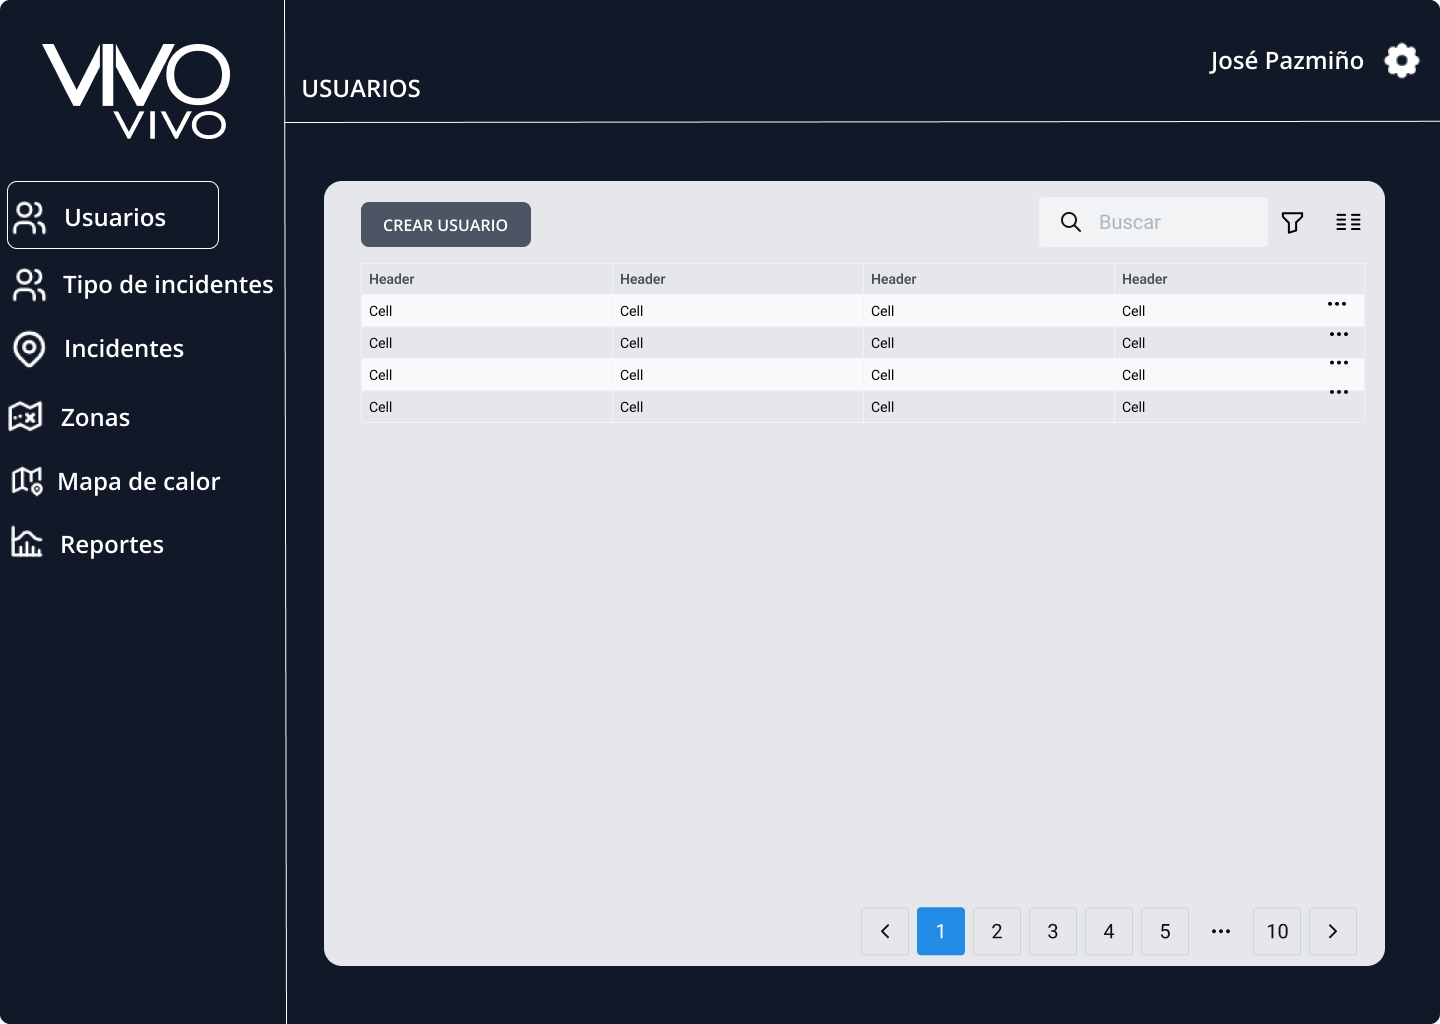
\includegraphics[width=0.6\textwidth]{chapters/III-resultados-y-discusion/resources/images/prototipo-tabla-usuarios-web.png}
    \caption{Prototipo de la interfaz de usuario web: Tabla de usuarios.}
    \label{fig:prototipo-tabla-usuarios-web}
\end{figure}

\begin{figure}[H]
    \centering
    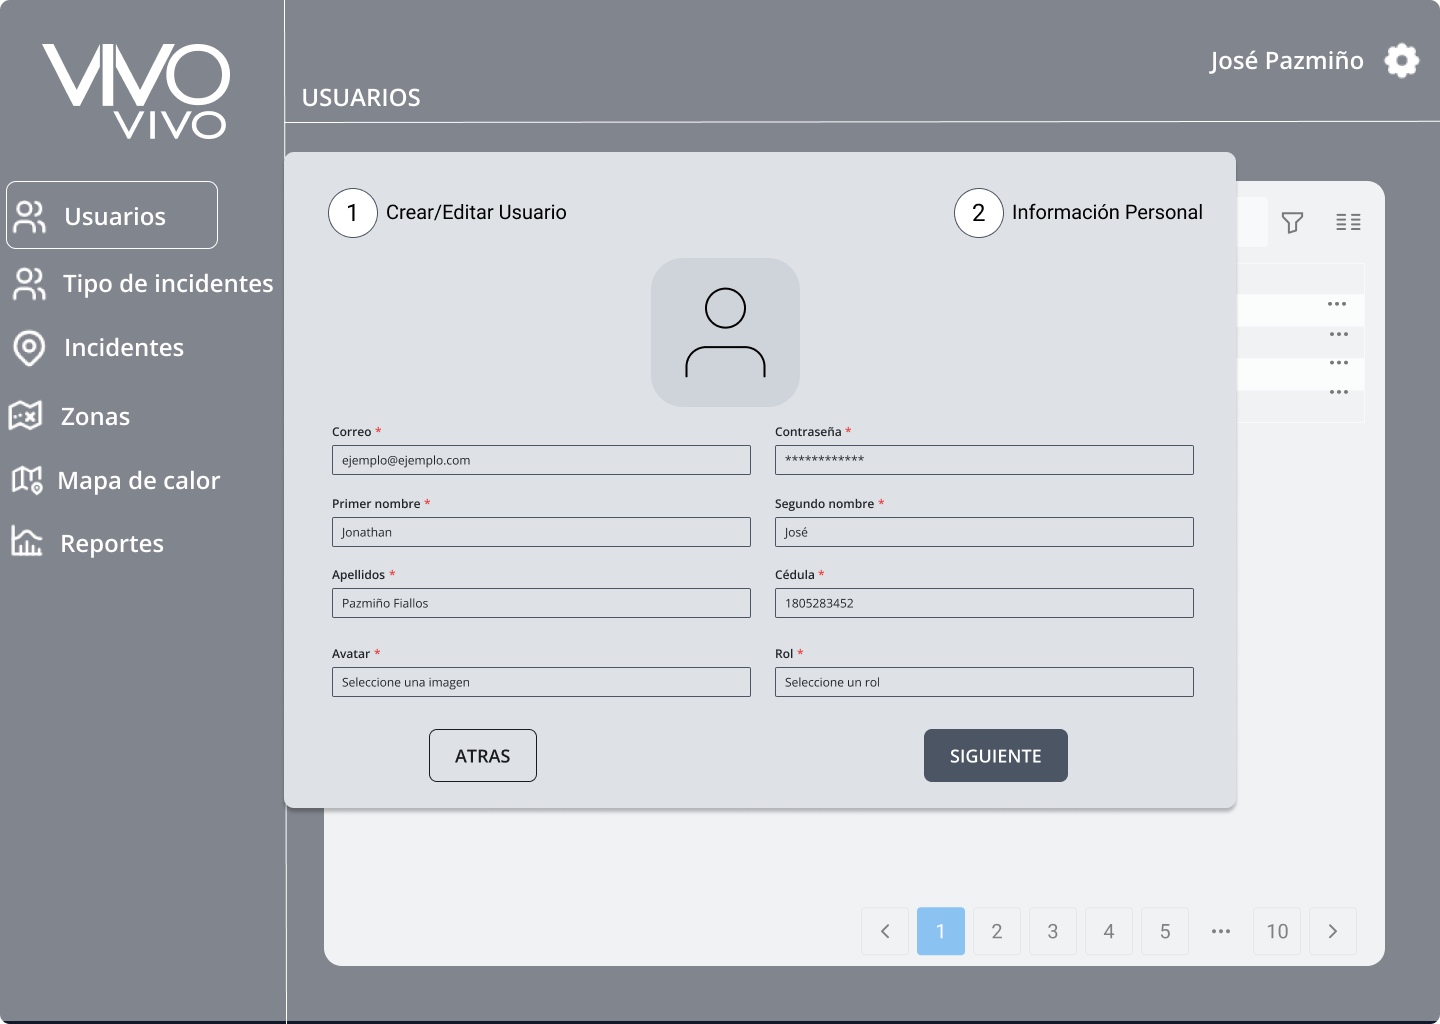
\includegraphics[width=0.6\textwidth]{chapters/III-resultados-y-discusion/resources/images/prototipo-formulario-usuario-web.png}
    \caption{Prototipo de la interfaz de usuario web: Formulario de usuario.}
    \label{fig:prototipo-formulario-usuario-web}
\end{figure}

Para la visualización de la información de los tipos de incidentes en el sistema web, se desarrolló una tabla de entradas, como se muestra en la Figura
\ref{fig:prototipo-tabla-tipos-incidentes-web}. Se propone un formulario de registro en el cual el usuario administrador puede ingresar la información
necesaria para crear un nuevo tipo de incidente, así como actualizar la información de un tipo de incidente existente y eliminar un tipo de incidente,
como se muestra en la Figura \ref{fig:prototipo-formulario-tipo-incidente-web}.

\begin{figure}[H]
    \centering
    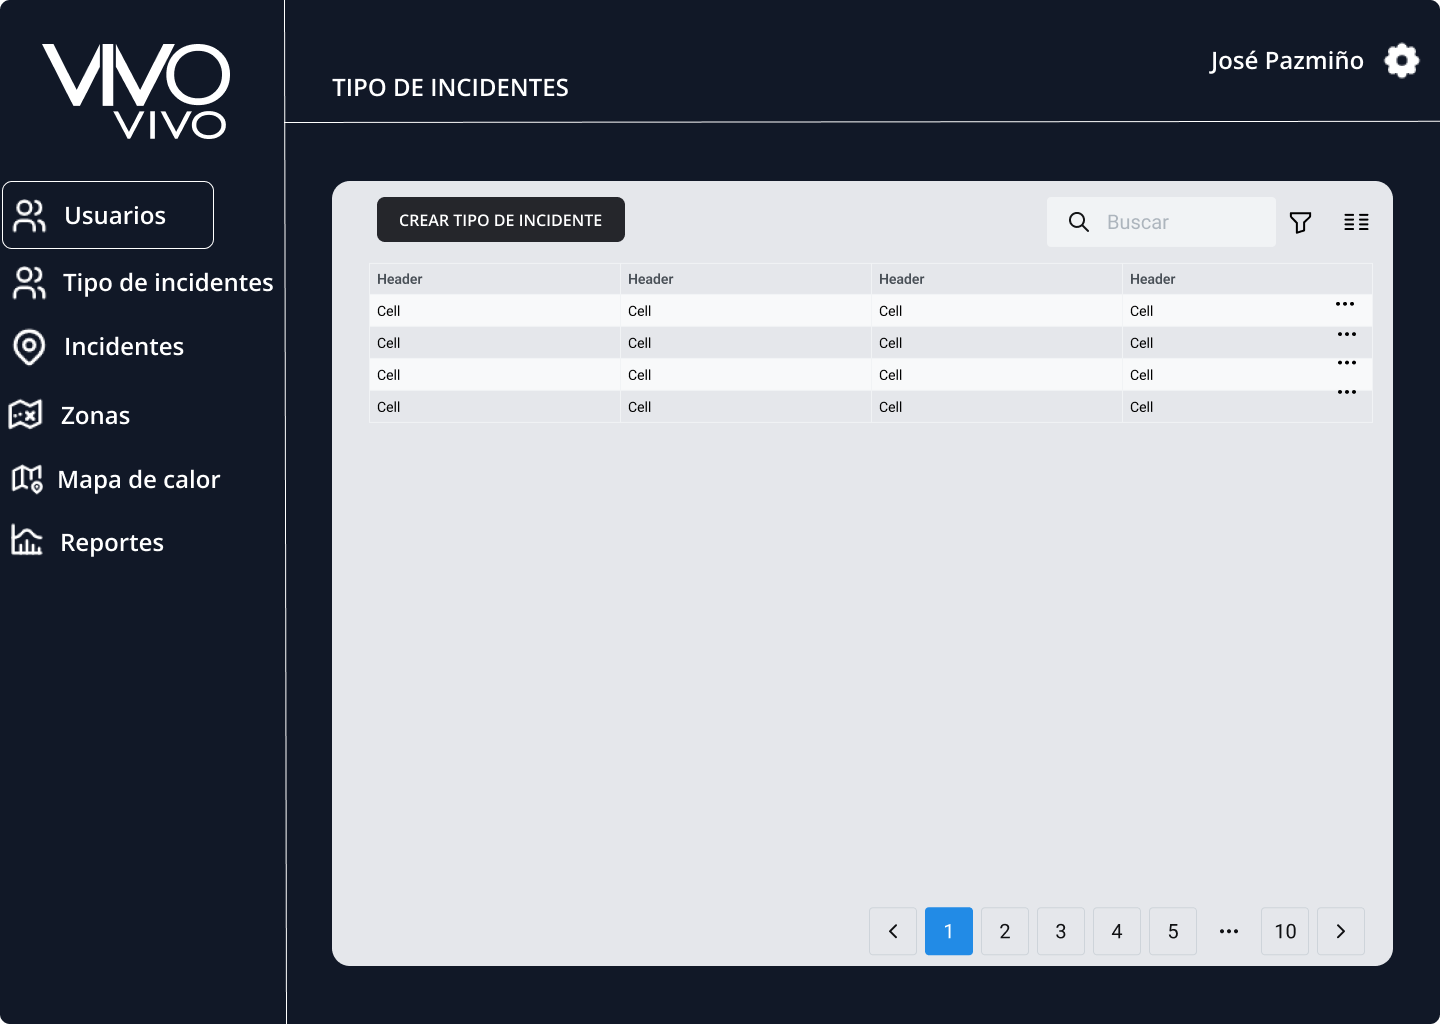
\includegraphics[width=0.6\textwidth]{chapters/III-resultados-y-discusion/resources/images/prototipo-tabla-tipos-incidentes-web.png}
    \caption{Prototipo de la interfaz de usuario web: Tabla de tipos de incidentes.}
    \label{fig:prototipo-tabla-tipos-incidentes-web}
\end{figure}

\begin{figure}[H]
    \centering
    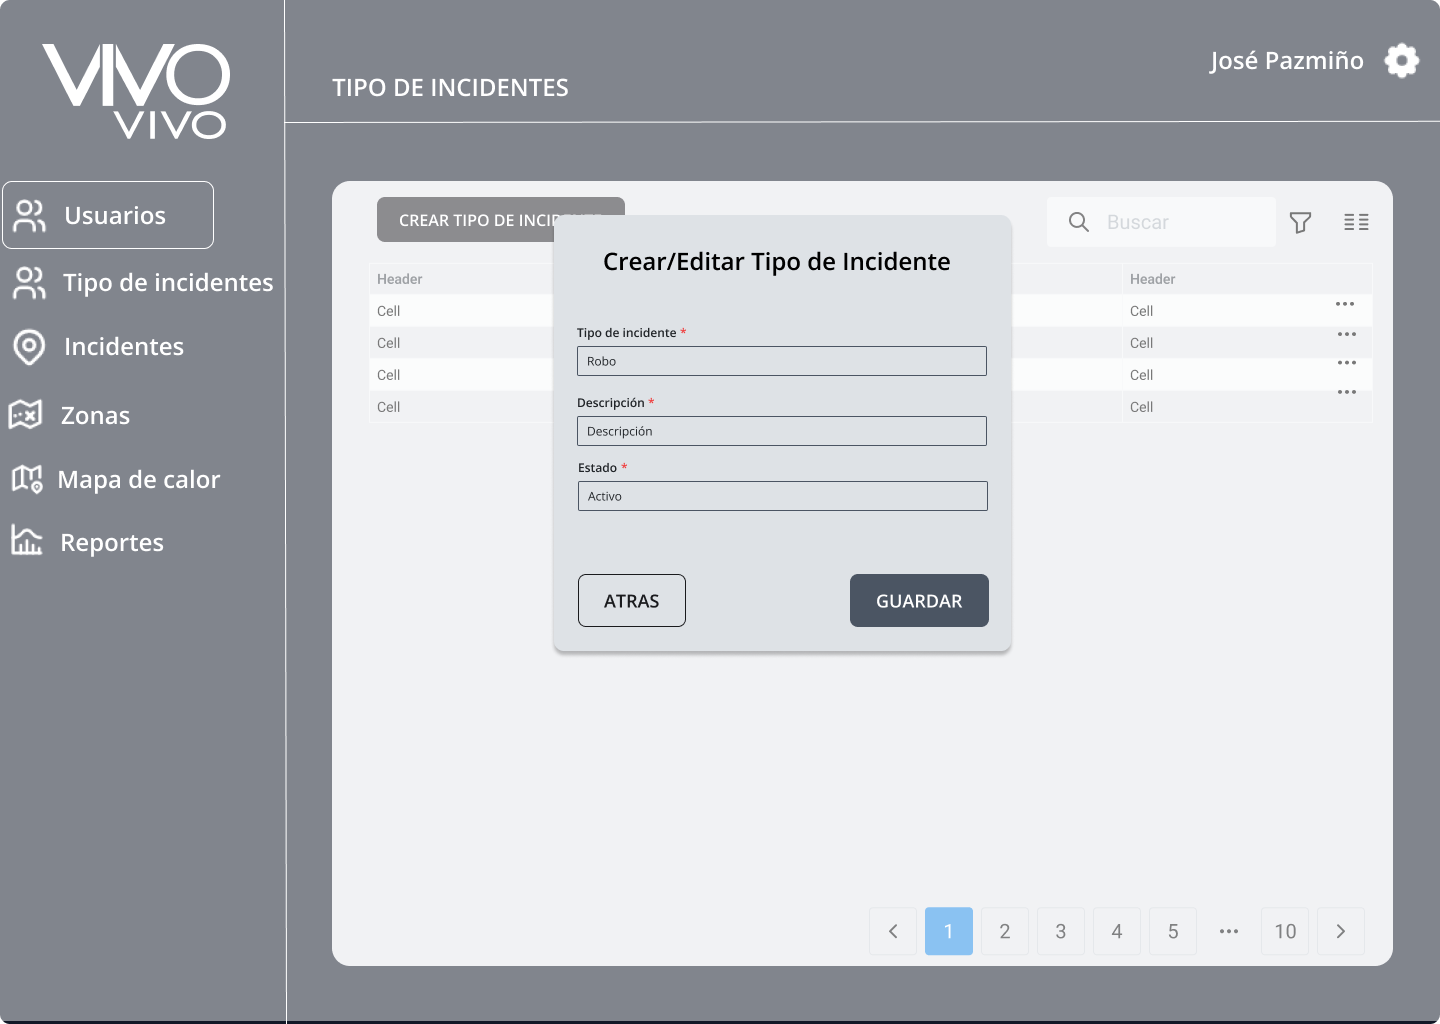
\includegraphics[width=0.6\textwidth]{chapters/III-resultados-y-discusion/resources/images/prototipo-formulario-tipo-incidente-web.png}
    \caption{Prototipo de la interfaz de usuario web: Formulario de tipo de incidente.}
    \label{fig:prototipo-formulario-tipo-incidente-web}
\end{figure}

En la Figura \ref{fig:prototipo-mapa-zonas-de-vigilancia-web} se muestra la pantalla de zonas de vigilancia, la cual permite al usuario administrador
visualizar las zonas de vigilancia mediante polígonos en un mapa interactivo.

\begin{figure}[H]
    \centering
    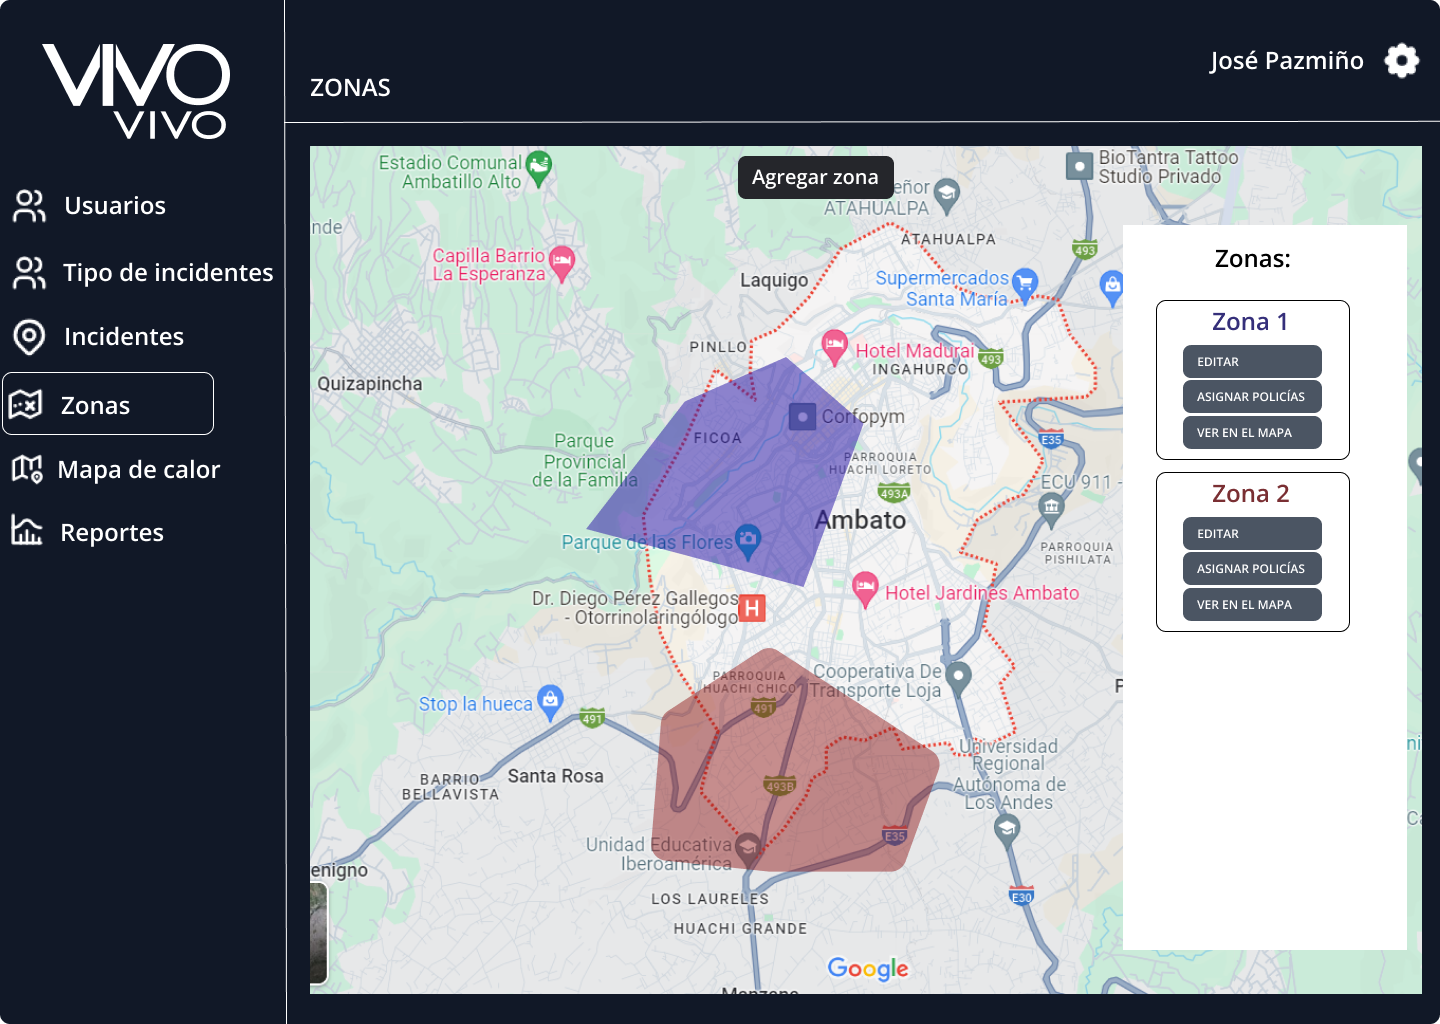
\includegraphics[width=0.6\textwidth]{chapters/III-resultados-y-discusion/resources/images/prototipo-mapa-zonas-de-vigilancia-web.png}
    \caption{Prototipo de la interfaz de usuario web: Mapa de zonas de vigilancia.}
    \label{fig:prototipo-mapa-zonas-de-vigilancia-web}
\end{figure}

Para la creación de zonas de vigilancia, se propone un formulario integrado con el mapa interactivo, el cual permite al usuario administrador
dibujar un polígono en el mapa para definir una zona de vigilancia, como se muestra en la Figura \ref{fig:prototipo-formulario-zona-vigilancia-web}.

\begin{figure}[H]
    \centering
    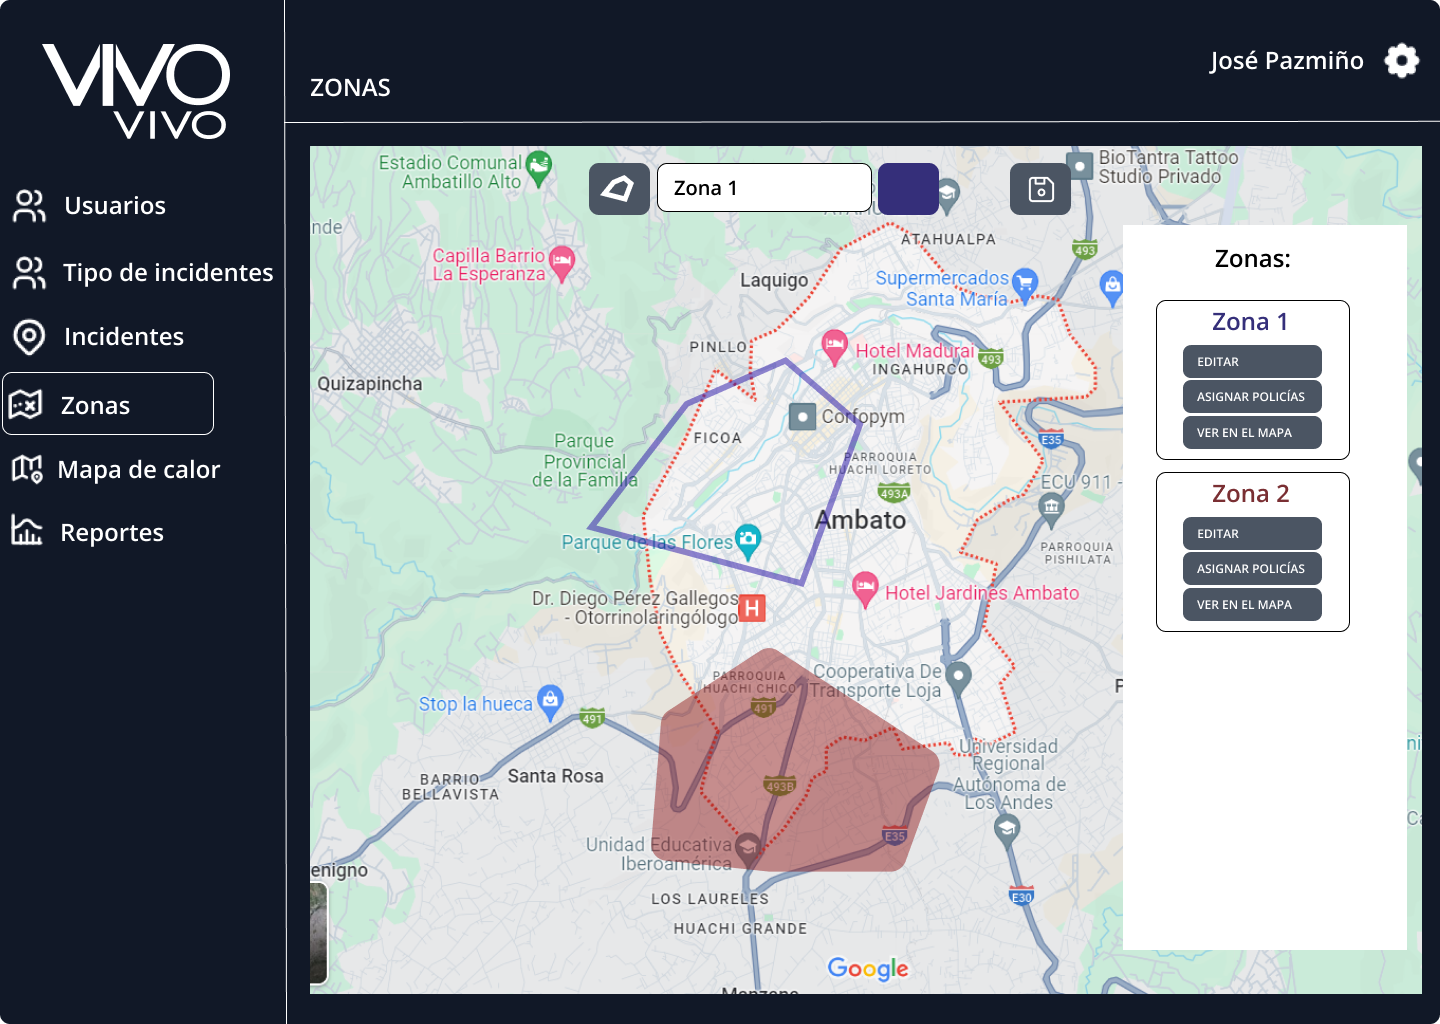
\includegraphics[width=0.6\textwidth]{chapters/III-resultados-y-discusion/resources/images/prototipo-formulario-zona-vigilancia-web.png}
    \caption{Prototipo de la interfaz de usuario web: Formulario de zona de vigilancia.}
    \label{fig:prototipo-formulario-zona-vigilancia-web}
\end{figure}

La pantalla de mapa de incidentes permite al usuario administrador visualizar los incidentes reportados en un mapa interactivo junto con la
ubicación en tiempo real de la víctima, como se muestra en la Figura \ref{fig:prototipo-mapa-incidentes-web}.

\begin{figure}[H]
    \centering
    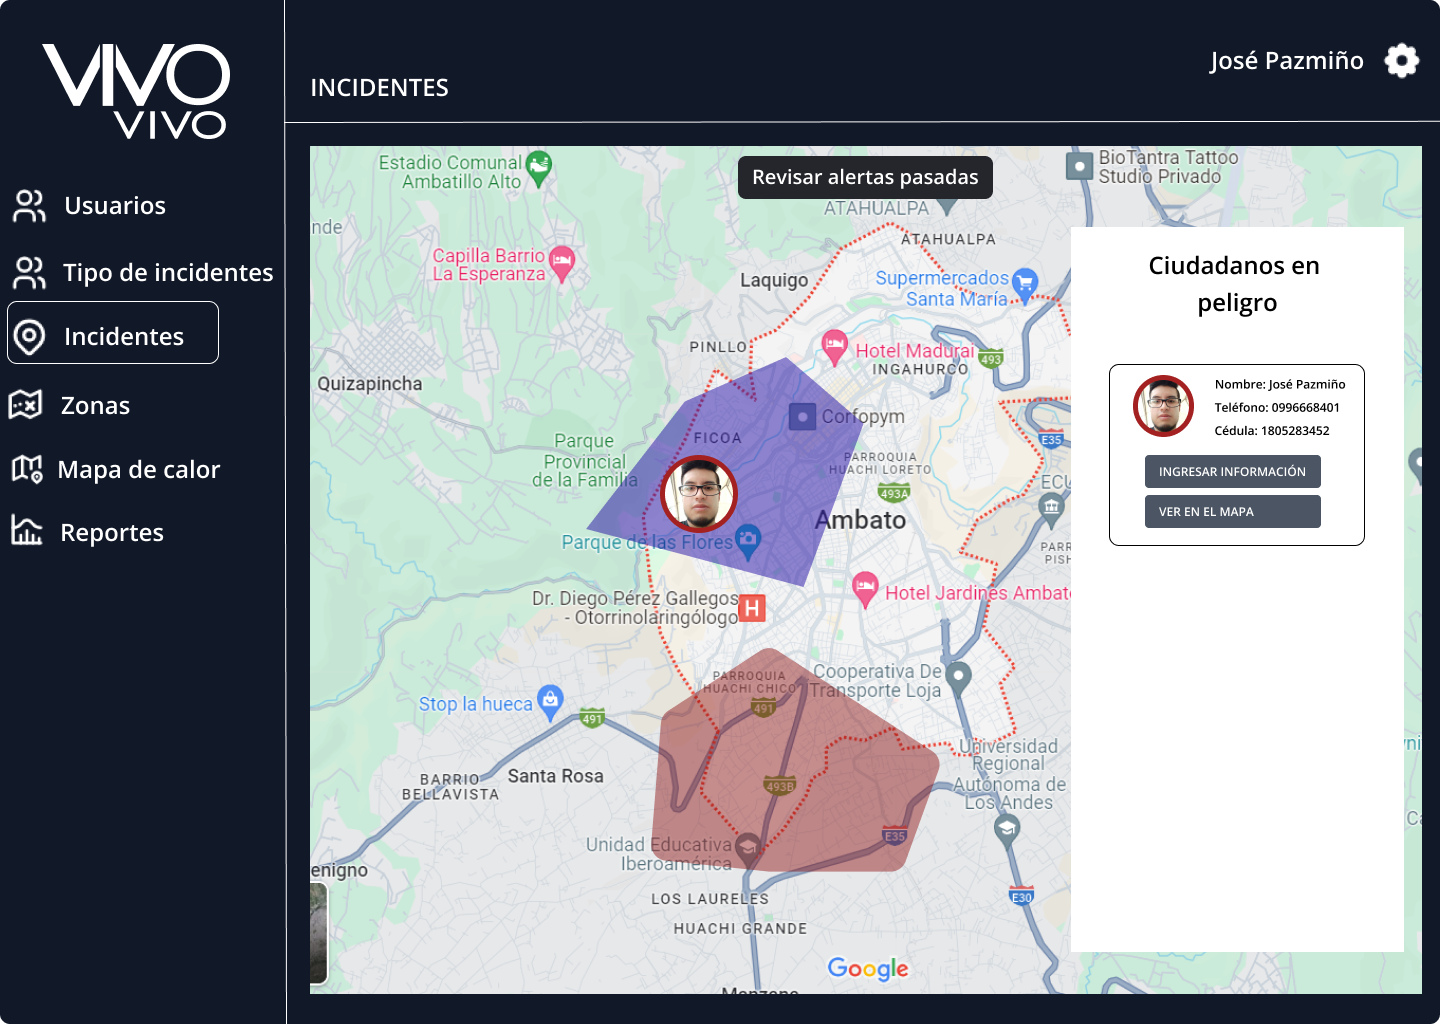
\includegraphics[width=0.6\textwidth]{chapters/III-resultados-y-discusion/resources/images/prototipo-mapa-incidentes-web.png}
    \caption{Prototipo de la interfaz de usuario web: Mapa de incidentes.}
    \label{fig:prototipo-mapa-incidentes-web}
\end{figure}

En la Figura \ref{fig:prototipo-mapa-de-calor-web} se muestra la pantalla de mapa de calor, la cual permite al usuario administrador visualizar
la densidad de incidentes reportados en un mapa interactivo mediante un gradiente de colores, así como filtrar los incidentes por tipo y fecha.

\begin{figure}[H]
    \centering
    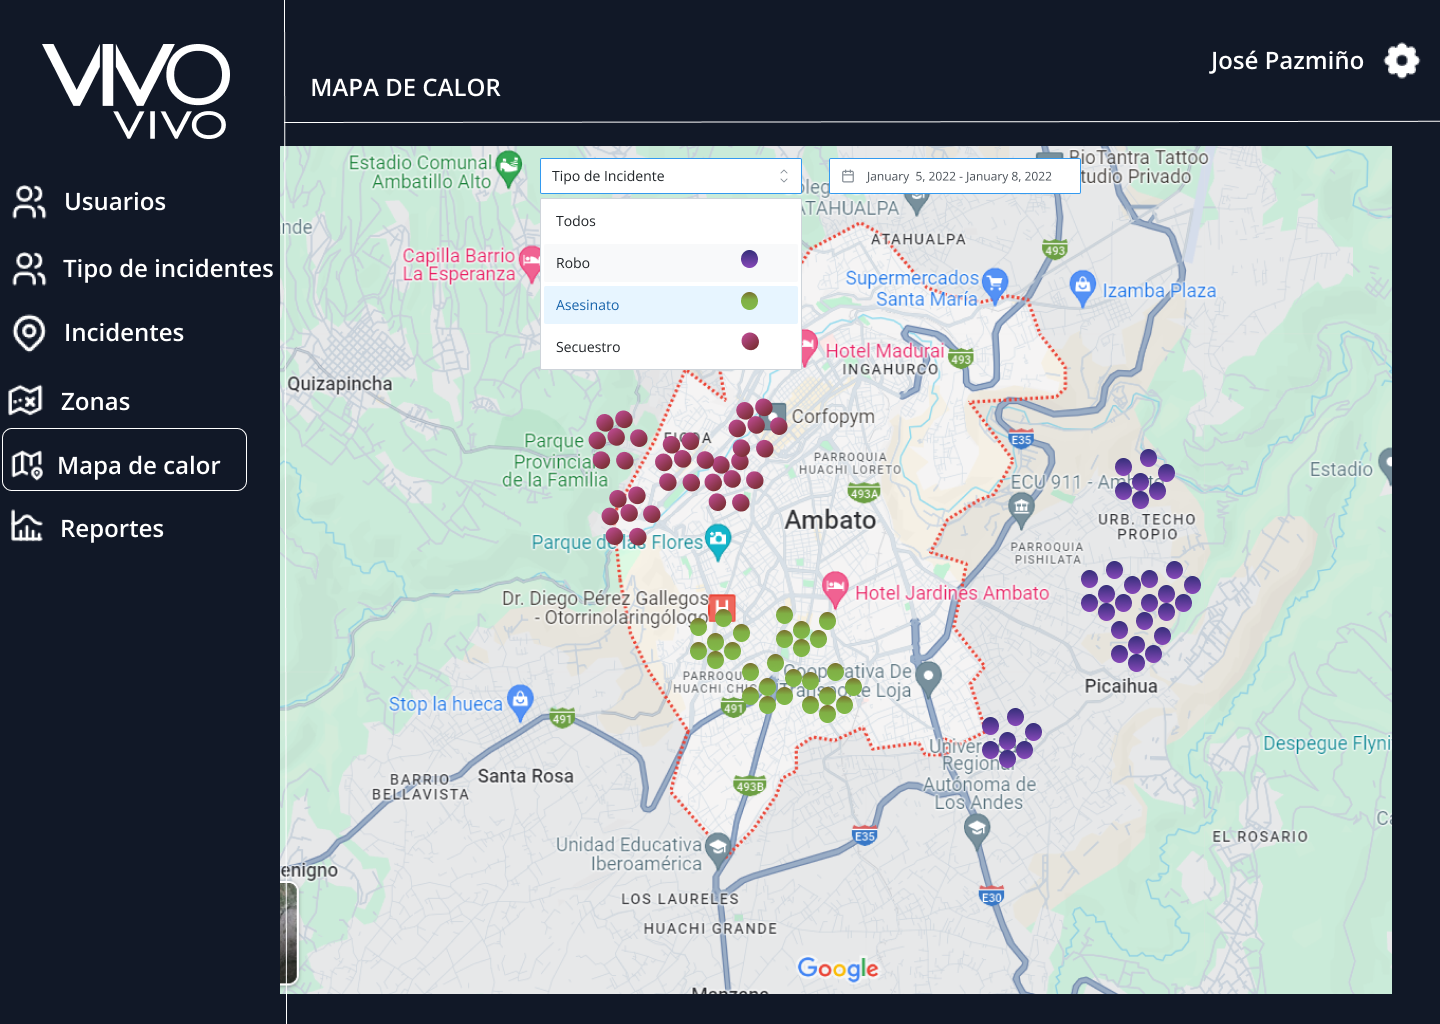
\includegraphics[width=0.6\textwidth]{chapters/III-resultados-y-discusion/resources/images/prototipo-mapa-de-calor-web.png}
    \caption{Prototipo de la interfaz de usuario web: Mapa de calor.}
    \label{fig:prototipo-mapa-de-calor-web}
\end{figure}

En la pantalla de reportería, el usuario administrador puede visualizar gráficos estadísticos de los incidentes reportados, tal como se muestra
en la Figura \ref{fig:prototipo-reporteria-web}.

\begin{figure}[H]
    \centering
    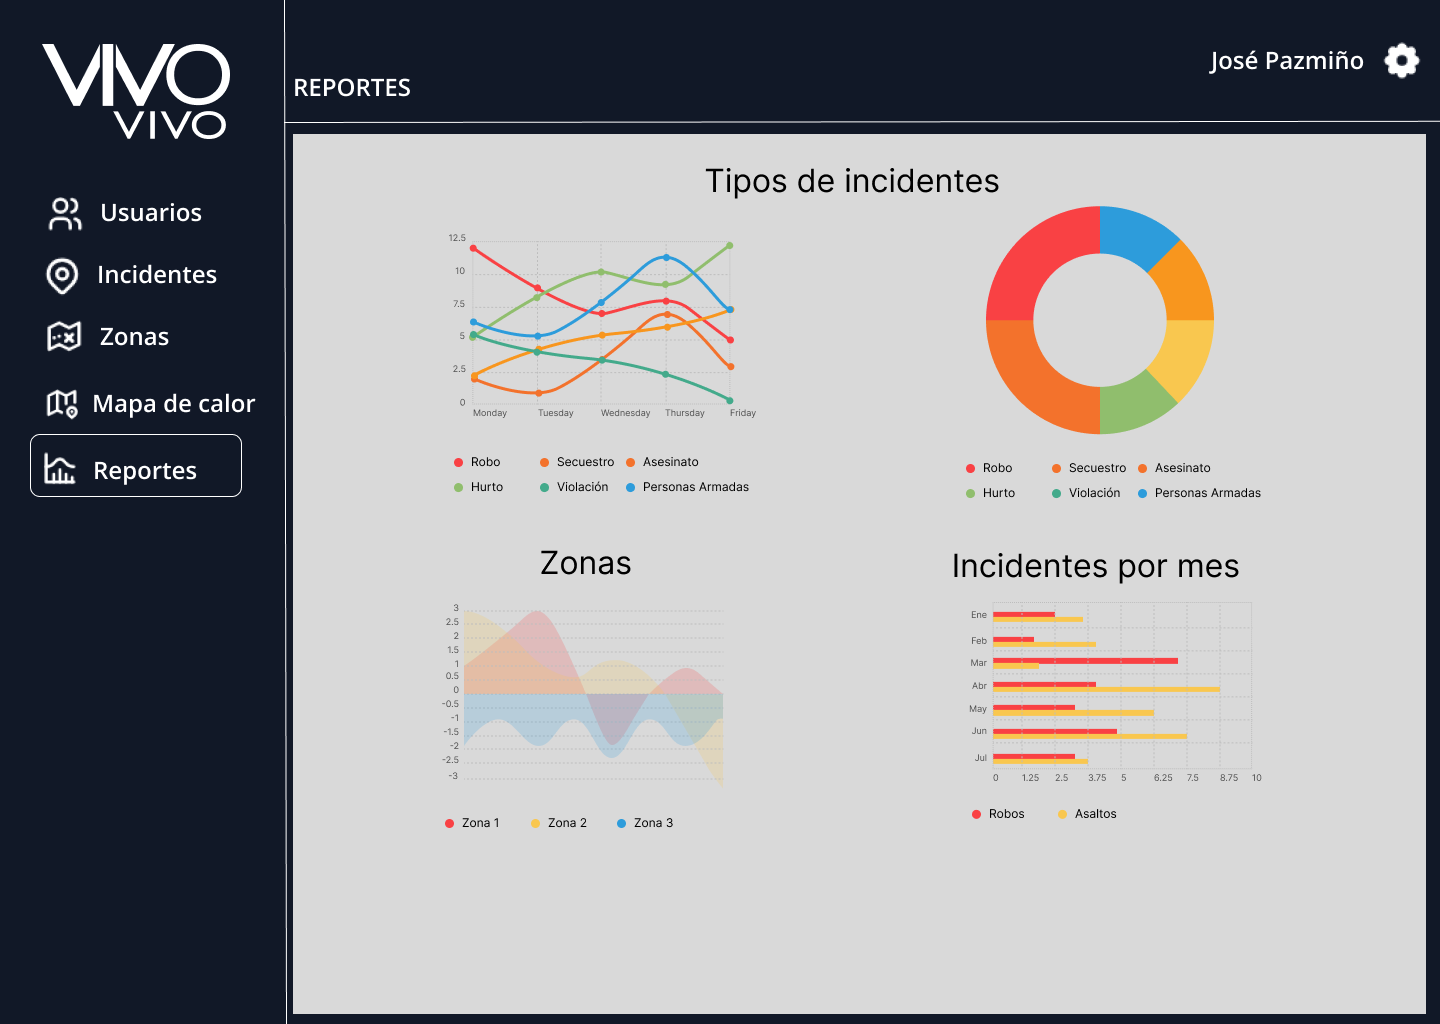
\includegraphics[width=0.6\textwidth]{chapters/III-resultados-y-discusion/resources/images/prototipo-reporteria-web.png}
    \caption{Prototipo de la interfaz de usuario web: Reportería.}
    \label{fig:prototipo-reporteria-web}
\end{figure}

\subsubsection{Prototipo de la interfaz de usuario móvil}
% TODO: REVISAR ORTOGRAFÍA
En la Figura \ref{fig:prototipo-inicio-sesion-mobile} se muestra la pantalla de inicio de sesión en la aplicación móvil, la cual se realiza mediante
el correo y contraseña del usuario.

\begin{figure}[H]
    \centering
    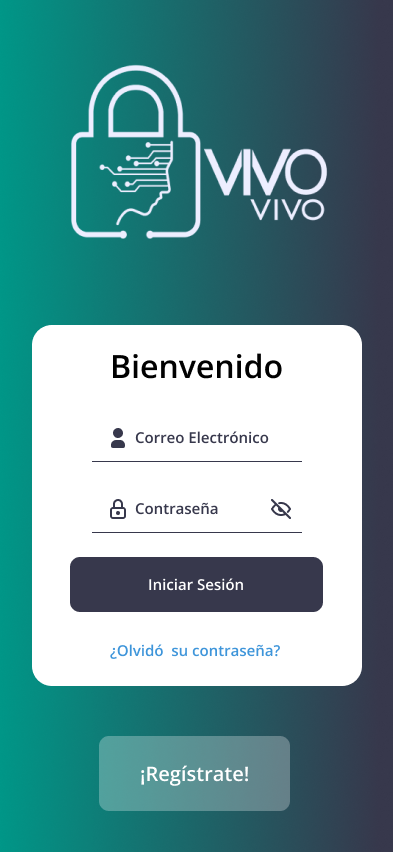
\includegraphics[width=0.3\textwidth]{chapters/III-resultados-y-discusion/resources/images/prototipo-inicio-sesion-mobile.png}
    \caption{Prototipo de la interfaz de usuario móvil: Inicio de sesión.}
    \label{fig:prototipo-inicio-sesion-mobile}
\end{figure}

Para el registro de usuarios se propone un formulario en el cual se ingresan una fotografía, nombres, apellidos, etnia, género, estado civil,
discapacidad en caso de presentarla y dirección, tal como se muestra en la Figura \ref{fig:prototipo-registro-mobile}.

\begin{figure}[H]
    \centering
    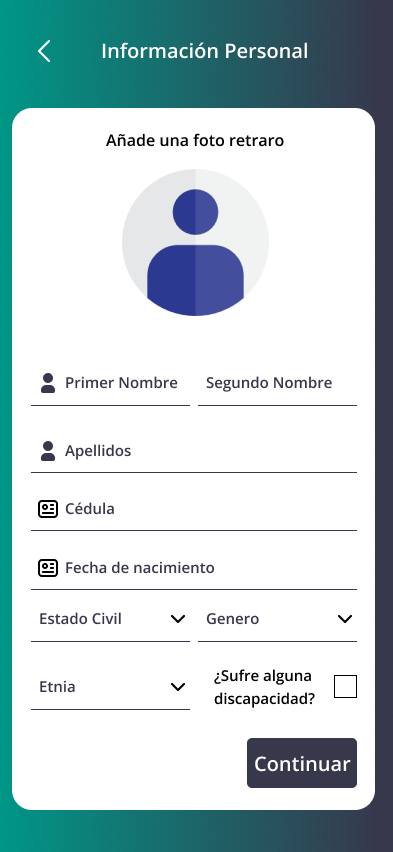
\includegraphics[width=0.3\textwidth]{chapters/III-resultados-y-discusion/resources/images/prototipo-registro-mobile.png}
    \caption{Prototipo de la interfaz de usuario móvil: Registro.}
    \label{fig:prototipo-registro-mobile}
\end{figure}

En la Figura \ref{fig:prototipo-recuperar-contrasena-mobile} se muestra la pantalla de recuperación de contraseña en la aplicación móvil, la cual se realiza
mediante el correo electrónico del usuario.

\begin{figure}[H]
    \centering
    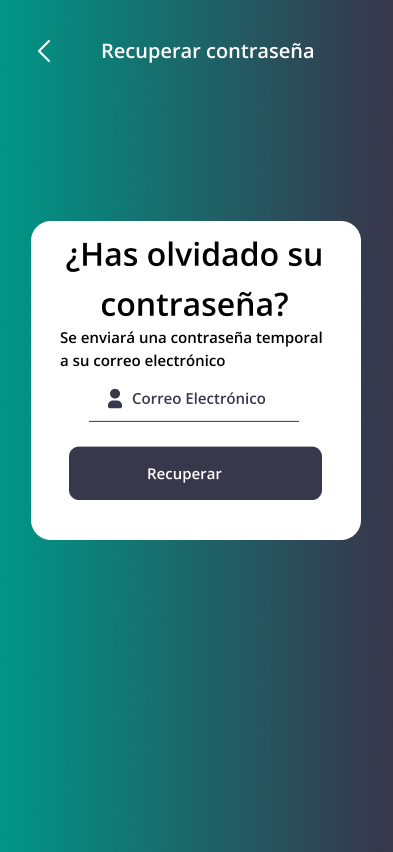
\includegraphics[width=0.3\textwidth]{chapters/III-resultados-y-discusion/resources/images/prototipo-recuperar-contrasena-mobile.png}
    \caption{Prototipo de la interfaz de usuario móvil: Recuperación de contraseña.}
    \label{fig:prototipo-recuperar-contrasena-mobile}
\end{figure}

Para la pantalla de inicio, se propone un botón de pánico que permite al usuario enviar una alerta de emergencia seleccionando el tipo de incidente y
presionando el botón durante 3 segundos para enviar la alerta. En la esquina superior derecha se encuentra el menú de opciones de la aplicación y en la
esquina superior izquierda se encuentra el botón de notificaciones de alertas de emergencia, como se muestra en la Figura \ref{fig:prototipo-inicio-mobile}.

\begin{figure}[H]
    \centering
    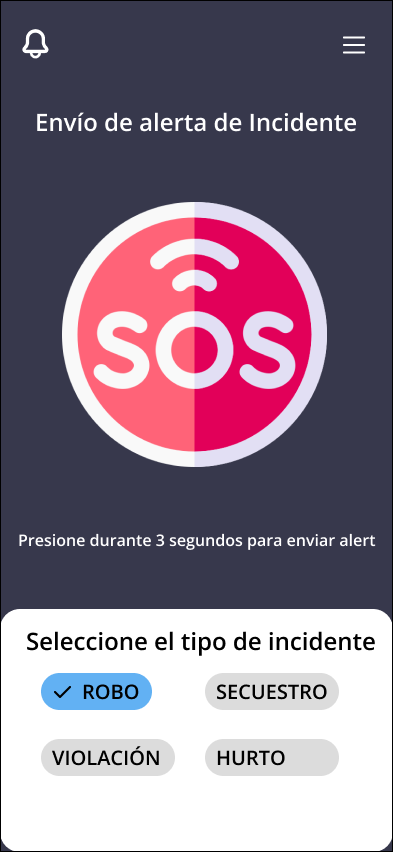
\includegraphics[width=0.3\textwidth]{chapters/III-resultados-y-discusion/resources/images/prototipo-inicio-mobile.png}
    \caption{Prototipo de la interfaz de usuario móvil: Inicio.}
    \label{fig:prototipo-inicio-mobile}
\end{figure}

En la Figura  \ref{fig:prototipo-alertas-mobile} se muestra la pantalla de alertas de emergencia, el usuario puede visualizar las alertas de emergencia
enviadas por los miembros del grupo familiar mediante una lista de alertas con la información de la persona y un botón para visualizar la ubicación
en tiempo real del incidente en un mapa interactivo como se puede observar en la Figura \ref{fig:prototipo-ubicacion-alerta-mobile}.

\begin{figure}[H]
    \centering
    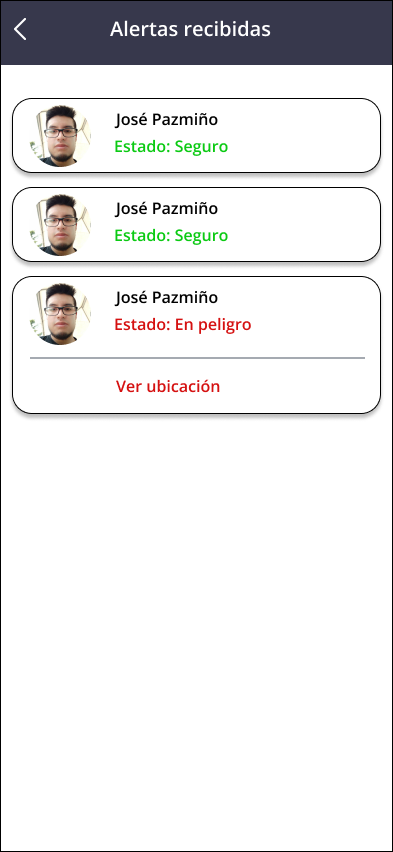
\includegraphics[width=0.3\textwidth]{chapters/III-resultados-y-discusion/resources/images/prototipo-alertas-mobile.png}
    \caption{Prototipo de la interfaz de usuario móvil: Alertas de emergencia.}
    \label{fig:prototipo-alertas-mobile}
\end{figure}

\begin{figure}[H]
    \centering
    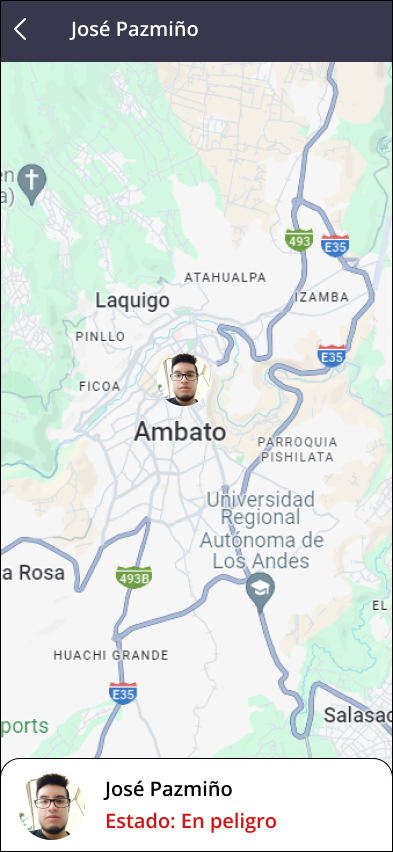
\includegraphics[width=0.3\textwidth]{chapters/III-resultados-y-discusion/resources/images/prototipo-ubicacion-alerta-mobile.png}
    \caption{Prototipo de la interfaz de usuario móvil: Ubicación de alerta.}
    \label{fig:prototipo-ubicacion-alerta-mobile}
\end{figure}

El menú de opciones de la aplicación móvil permite al usuario gestionar su grupo familiar, cambiar su contraseña y cerrar sesión, como se muestra
en la Figura \ref{fig:prototipo-menu-mobile}.

\begin{figure}[H]
    \centering
    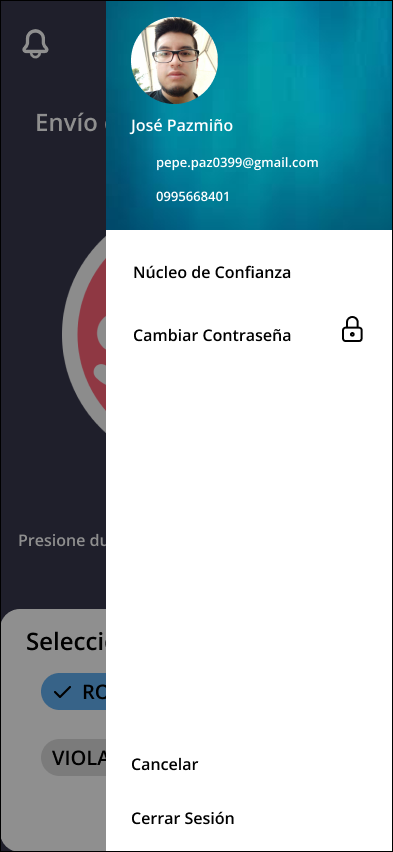
\includegraphics[width=0.3\textwidth]{chapters/III-resultados-y-discusion/resources/images/prototipo-menu-mobile.png}
    \caption{Prototipo de la interfaz de usuario móvil: Menú.}
    \label{fig:prototipo-menu-mobile}
\end{figure}

Para la gestión de grupos familiares, se propone una pantalla en la cual el usuario puede visualizar los miembros de su grupo familiar y agregar
nuevos miembros, como se muestra en la Figura \ref{fig:prototipo-grupo-familiar-mobile}. Al agregar un nuevo miembro, se muestra un formulario
en el cual se puede buscar un usuario por su cédula de identidad y agregarlo al grupo familiar, como se muestra en la Figura \ref{fig:prototipo-agregar-miembro-mobile}.

\begin{figure}[H]
    \centering
    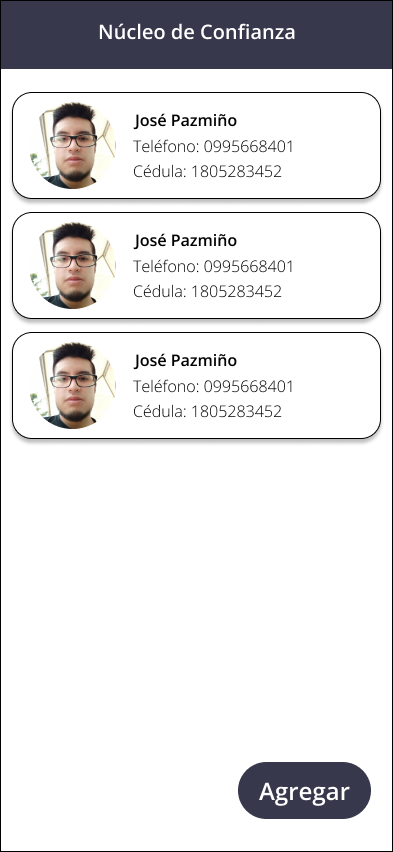
\includegraphics[width=0.3\textwidth]{chapters/III-resultados-y-discusion/resources/images/prototipo-grupo-familiar-mobile.png}
    \caption{Prototipo de la interfaz de usuario móvil: Grupo familiar.}
    \label{fig:prototipo-grupo-familiar-mobile}
\end{figure}

\begin{figure}[H]
    \centering
    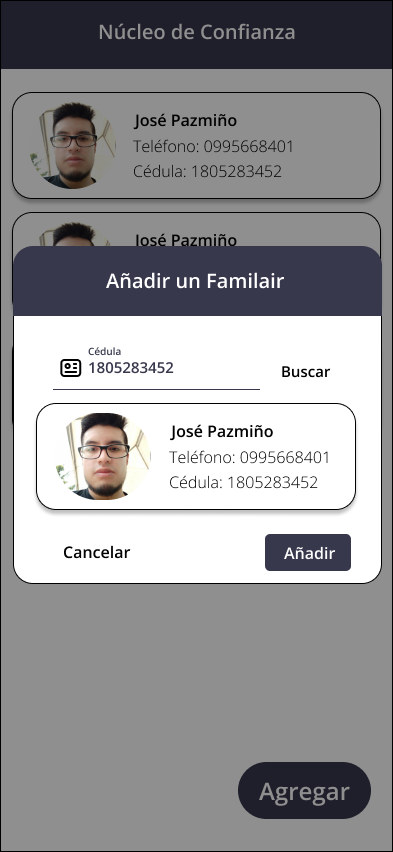
\includegraphics[width=0.3\textwidth]{chapters/III-resultados-y-discusion/resources/images/prototipo-agregar-miembro-mobile.png}
    \caption{Prototipo de la interfaz de usuario móvil: Agregar miembro.}
    \label{fig:prototipo-agregar-miembro-mobile}
\end{figure}

En la Figura \ref{fig:prototipo-cambiar-contrasena-mobile} se muestra la pantalla para cambiar la contraseña en la aplicación móvil. El usuario
debe ingresar su contraseña actual, la nueva contraseña y confirmar la nueva contraseña para realizar el cambio.

\begin{figure}[H]
    \centering
    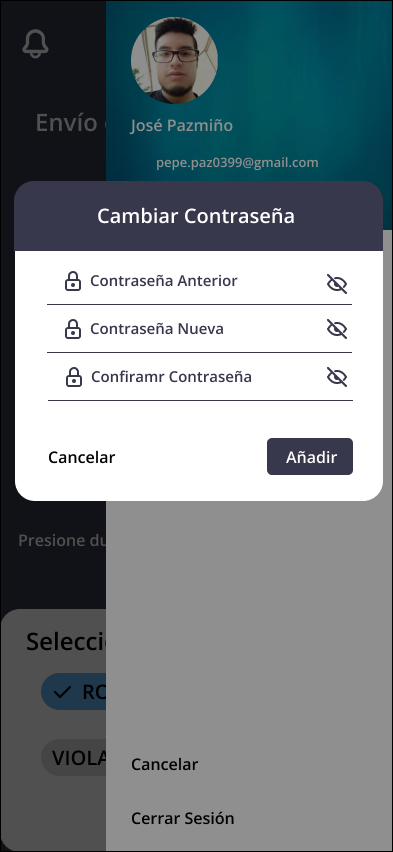
\includegraphics[width=0.3\textwidth]{chapters/III-resultados-y-discusion/resources/images/prototipo-cambiar-contrasena-mobile.png}
    \caption{Prototipo de la interfaz de usuario móvil: Cambiar contraseña.}
    \label{fig:prototipo-cambiar-contrasena-mobile}
\end{figure}

\subsection{Construcción}

